\documentclass[output=paper]{langscibook}
\ChapterDOI{10.5281/zenodo.15148186}
\author{Shigeko Shinohara\orcid{}\affiliation{Laboratoire de Phonétique et Phonologie, Université Sorbonne Nouvelle, CNRS} and Qandeel Hussain\orcid{}\affiliation{Universität Bamberg; University of Toronto; North Carolina State University} and Angélique Amelot\orcid{}\affiliation{Laboratoire de Phonétique et Phonologie, Université Sorbonne Nouvelle, CNRS}}
\title[Correlates of word-initial voiceless nasal geminates in Ikema Miyako]{Aerodynamic and acoustic correlates of word-initial voiceless nasal geminates in Ikema Miyako Ryukyuan}
\abstract{This study investigates the voiceless nasal sounds of the Ikema dialect of Miyako Ryukyuan, which is a severely endangered language spoken on the Miyako Islands in Japan. Miyako Ryukyuan exhibits a variety of geminate consonants, but Ikema is the only Miyako dialect that has developed voiceless nasal consonants as part of its word-initial geminate inventory. To investigate the voicing contrast of nasals, we explored aerodynamic and acoustic recordings from ten speakers. Acoustic measures (fundamental frequency and H1*-H2*) aimed to find voicing cues in the following vowel. Our results indicate that the airflow patterns of Ikema voiceless nasals are similar to those of Burmese, except that the voicing rate is higher in Ikema. Acoustic measures do not reveal any enhancing cue of the voicing feature. This result might be due to the longer voiced duration in the voiceless nasals, which our study also confirmed.

\keywords{voiceless nasals, nasal airflow, Ikema Miyako Ryukyuan, endangered language description}}
\IfFileExists{../localcommands.tex}{
  \addbibresource{../localbibliography.bib}
  \usepackage{tabularx, multicol, multirow, longtable}
\usepackage{url}
\urlstyle{same}

\usepackage{orcidlink}
\definecolor{orcidlogocol}{cmyk}{0,0,0,1}
\RenewDocumentCommand{\LinkToORCIDinAffiliations}{ +m }
  {%
    \orcidlink{#1}\,%
  }
\SetupAffiliations{orcid placement=before}

\usepackage{siunitx}
\sisetup{detect-weight=true, detect-family=true, group-digits=none}

\usepackage{mathtools}
\usepackage{langsci-optional}
\usepackage{langsci-lgr}
\usepackage{langsci-gb4e}

\usepackage{stmaryrd}
\usepackage[capitalize]{cleveref}
\babelfont[macedonian]{rm}[Language=Macedonian,ItalicFont=LibertinusSerif-Italic.otf]{LibertinusSerif-Regular.otf}
\usepackage{eqparbox}
\usepackage[autostyle]{csquotes}
\usepackage[linguistics]{forest}

\usetikzlibrary{positioning, matrix}
\usepackage[glosses,inline]{leipzig}
\PassOptionsToPackage{xindy,toc,nopostdot}{glossaries}
\usepackage{glossary-inline}
\setglossarystyle{inline}
\makeglossaries

\usepackage{phonrule}
\usepackage{threeparttable}


\usepackage{textcomp,gensymb}


\usepackage[preservefont]{tipauni}

\usepackage[normalem]{ulem}

\usepackage{enumitem} %so lists aren't ugly
	
\usepackage{threeparttable}	%allows tables with tablenotes. note marks: †‡
	\makeatletter 
	\g@addto@macro\TPT@defaults{\footnotesize} 
	\makeatother

\usepackage{colortbl}
	\definecolor{Pink}{rgb}{0.96, 0.76, 0.76} 
	\definecolor{PaleBlue}{rgb}{0.67, 0.9, 0.93}
	\definecolor{carolinablue}{rgb}{0.6, 0.73, 0.89}
	\definecolor{goldenyellow}{rgb}{1.0, 0.87, 0.0}
	\definecolor{Orange}{rgb}{1.0, 0.66, 0.07}
	\definecolor{puce}{rgb}{0.8, 0.53, 0.6}
	\definecolor{turquoisegreen}{rgb}{0.63, 0.84, 0.71}


% add all extra packages you need to load to this file
\usepackage{langsci-textipa}
\usepackage{vowel}
\usepackage{textgreek}

% \usepackage{langsci-branding}
% \usepackage{subcaption}
\usepackage{subfigure}

\usepackage{tabto}


\usetikzlibrary{tikzmark}
\usepackage{pgfplots}


\newfontfamily\tibetan{NotoSerifTibetan-Regular.ttf}
\usepackage{langsci-branding}
\usepackage{hyphenat}

\usepackage{accents}

  \renewcommand{\lsChapterFooterSize}{\footnotesize}

\makeatletter
\let\thetitle\@title
\let\theauthor\@author
\makeatother

\newcommand{\togglepaper}[1][0]{
   \bibliography{../localbibliography}
   \papernote{\scriptsize\normalfont
     \theauthor.
     \titleTemp.
     To appear in:
     Natalia Kuznetsova, Cormac Anderson \& Shelece Easterday (ed.).
     Rarities in phonetics and phonology.tex.
     Berlin: Language Science Press. [preliminary page numbering]
   }
   \pagenumbering{roman}
   \setcounter{chapter}{#1}
   \addtocounter{chapter}{-1}
}

\newbool{bookcompile}
\booltrue{bookcompile}
\newcommand{\bookorchapter}[2]{\ifbool{bookcompile}{#1}{#2}}

\newcommand{\textarab}[1]{\RL{\arabicfont #1}}

\newcommand\mb[1]{\eqparbox[t]{examples}{#1}\hspace{1em}}
\newcommand\mbi[1]{\mb{#1}}
\newcommand{\twe}[3]{\mbi{#1}\eqparbox[t]{orths}{\emph{#2}}\hspace{1em}`#3'\hspace{1em}} % three-way example
\providecommand\glottocode[1]{[\href{https://glottolog.org/resource/languoid/id/#1}{#1}]}
\newcommand{\phonreal}[1]{\ensuremath{\llbracket}#1\ensuremath{\rrbracket}}

\DeclareRobustCommand\dash{\unskip\nobreak\thinspace\textendash\allowbreak\thinspace\ignorespaces}

\forestset{minus/.style={edge label={node[midway, left] {\ensuremath{-}\hspace*{2mm}}}},
plus/.style={edge label={node[midway, right] {\hspace*{2mm}\ensuremath{+}}}}}
\providecommand\ipa[1]{#1}


\newcommand{\tone}[1]{\textsuperscript{#1}}

\newcommand{\orthog}[1]{\textit{#1}}
\newcommand{\gloss}[1]{`#1'}

\newcommand{\glottolog}[1]{\texttt{\href{https://glottolog.org/resource/languoid/id/#1}{#1}}}

\newcolumntype{O}{>{\itshape }l<{}}
\newcolumntype{G}{>{`}l<{'}}

\newcounter{tabsubcounter}
\newcommand{\tablecounter}{\setcounter{tabsubcounter}{0}}
\newcommand{\TC}{\stepcounter{tabsubcounter}\alph{tabsubcounter}.}

\usetikzlibrary{chains,positioning,calc,decorations.markings}
\tikzset{
	seg/.style={text height=0.6em, text depth=0.3em},
	moraic-structure/.style={xscale=0.6,yscale=1.1, text height=0.65em,text depth=0.25em},
 }

%05_Culhane_Edwards
%%%%%%%%%%%%%%%%%%%%%%%%%%%%%%%%
%%	Symbols and Characters  	%%
%%%%%%%%%%%%%%%%%%%%%%%%%%%%%%%% αβσµ

\newcommand{\tl}{\char`~}						%middle tilde ~
\renewcommand{\Q}{\textquotesingle}		%straight apostrophe444
\newcommand{\ra}{→} 								%right arrow ->
\newcommand{\0}{∅} 									%zero symbol
\newcommand{\gap}{\textunderscore} 	%underscore
%\renewcommand{\j}{ʤ}								%dezh digraph
\newcommand{\syll}{σ}								%lowercase sigma medial form
\newcommand{\wrd}{ω}								%lowercase omega
\newcommand{\ft}{φ}									%lowercase phi
\newcommand{\gw}{gʷ}								%g with superscript w
\newcommand{\B}{β}									%voiced bilabial fricative
\newcommand{\hp}{\hphantom}					%space equal to width of argument
\newcommand{\it}{\textit}	%italics

%%%%%%%%%%%%%%%%%%%%%%%%%%%%%%%%
%%	Font Styles & Formatting	%%
%%%%%%%%%%%%%%%%%%%%%%%%%%%%%%%%

\definecolor{DarkBlue}{RGB}{0,0,130}										%dark blue colour
% \newcommand{\ve}[1]{\textcolor{DarkBlue}{\textit{#1}}}	%vernacular text
\newcommand{\ve}[1]{{\textit{#1}}}	%vernacular text
\definecolor{DarkRed}{RGB}{150,0,0}											%dark red colour
% \newcommand{\tbr}[1]{\textcolor{DarkRed}{\textbf{#1}}}	%Bold red text
\newcommand{\tbr}[1]{{\textbf{#1}}}	%Bold red text
%\renewcommand{\it}{\textit}																%italics
\newcommand{\tsc}{\textsc}															%small caps
\newcommand{\sub}{\textsubscript}												%subscript
\newcommand{\su}{\textsuperscript}											%superscript

%%%%%%%%%%%%%%%%%%%%%%%%%%%%%%%%%%%%%%%%%%%%%%%%%%%%
%% Tables %% Tables %% Tables %% Tables %% Tables %%
%%%%%%%%%%%%%%%%%%%%%%%%%%%%%%%%%%%%%%%%%%%%%%%%%%%%

% \newcommand{\mc}{\multicolumn}									%multicolumn
% \newcommand{\st}[1]{\setlength{\tabcolsep}{#1}}	%reduce column width in tables
%
%%%%%%%%%%%%%%%%%%%%%%%%%%%%%%%%
%%    Cross   References      %%
%%%%%%%%%%%%%%%%%%%%%%%%%%%%%%%%

% \def\Plus{\texttt{+}}
% \def\Minus{\texttt{-}}
% \newcommand{\GS}{ʔ}
% \def\SH{ʃ}
% \newcommand{\TSH}{ʧ}
% \def\ZH{ʒ}
% \def\DZH{ʤ}
% \def\:{ː}
% \def\UP{\textsuperscript}
% \def\rs{ʂ}
% \newcommand{\rn}{ɳ}
% \def\rt{ʈ}
% \def\tllr{ɺ}
% \newcommand{\Bb}{β}
% \def\Eps{ɛ}
% \def\Oo{ɔ}
% \def\Gm{ɣ}
% \def\NG{ŋ}
% \def\barU{ʉ}
\newcommand{\CM}{\ding{51}}
\newcommand{\XM}{\ding{53}}
% \newcommand{\tap}{ɾ}
% \def\darkL{ɫ}
% \def\schwa{ə}
%
% \def\BUL{\textbullet}


%%%%%%%%%%%%%%
%					%
%	Secondaries		%
%					%
%%%%%%%%%%%%%%
%	Post
\newcommand{\Post}[2]{#1\textsuperscript{#2}}
%	Pre
\newcommand{\Pre} [2] {\textsuperscript{#1}#2}
%	Undertilde
\newcommand{\utilde}[1]{\ensuremath{\smash{\underset{\mathclap{\sim}}{\text{#1}}}}}
%	Devoiced
% \newcommand{\VCLS}[1]{\textsubring{#1}}
%%%%%%%%%%%
%				%
%	Definitions		%
%	Markup		%
%				%
%%%%%%%%%%%
% \def\->{$\rightarrow$}
% \def\__{\underline{\hspace{1em}}}
\def\NoPoss{\cellcolor{gray!30}}

\newcommand{\VOICELESS}{\textsc{voiceless}}
\newcommand{\VOICED}{\textsc{voiced}}
\newcommand{\tablenote}[2][1]{\parbox{#1\textwidth}{\footnotesize\raggedright #2}}

\newcommand{\appref}[1]{Appendix~\ref{#1}}
\renewcommand{\sectref}[1]{Section~\ref{#1}}


\newcommand{\dobuibox}[5]{#1\\[-1.1em]
\hspace*{-.8cm}
 \begin{tabularx}{.9\textwidth}{@{}lQQ@{}}
       &  {oral} &  {nasal} \\
       \midrule
     {controlled} &\parbox[t]{4cm}{\raggedright  #2} & \parbox[t]{4cm}{\raggedright #3} \\
     \tablevspace
     {ballistic} &\parbox[t]{4cm}{\raggedright  #4} & \parbox[t]{4cm}{\raggedright  #5} \\
 \end{tabularx}
}

\newfontfamily\VdottildeFont{LibertinusVdottilde.otf}

\newcommand{\Vdottilde}{{\VdottildeFont V̰̣}}

% \renewcommand{\keywords}[1]{\textbf{#1}}

  %% hyphenation points for line breaks
%% Normally, automatic hyphenation in LaTeX is very good
%% If a word is mis-hyphenated, add it to this file
%%
%% add information to TeX file before \begin{document} with:
%% %% hyphenation points for line breaks
%% Normally, automatic hyphenation in LaTeX is very good
%% If a word is mis-hyphenated, add it to this file
%%
%% add information to TeX file before \begin{document} with:
%% %% hyphenation points for line breaks
%% Normally, automatic hyphenation in LaTeX is very good
%% If a word is mis-hyphenated, add it to this file
%%
%% add information to TeX file before \begin{document} with:
%% \include{localhyphenation}
\hyphenation{
    af-fri-cates
    al-ve-o-pal-a-tal
    Ama-nu-ban
    Ara-wak-an
    Árna-son
    Ber-ber
    can-di-dates
    Cam-er-oon
    Chi-nan-tec
    Chir-ko-va
    Crai-o-ve-a-nu
    di-chot-o-my
    Ec-ua-do-rian
    Ec-ua-dor
    elec-tro-glot-to-gra-phy
    Faro-ese
    Ike-ma
    Kuznet-sova
    Mes-kwa-ki
    Mio-ma-fo
    mono-mor-aic
    Ne-ca-xa
    Oto-man-gue-an
    par-a-digm
    post-as-pi-rat-ed
    post-as-pi-ra-tion
    pre-as-pi-rat-ed
    pre-as-pi-ra-tion
    pros-o-dic
    pros-o-dies
    re-con-struc-table
    Sheh-ret
    Svan-tes-son
    Ta-ras-can
    Tórs-havn
    Ural-ic
    epen-the-sis
    Anin-dil-yak-wa
    Mi-nyag
    Na-ka-ma
}

\hyphenation{
    af-fri-cates
    al-ve-o-pal-a-tal
    Ama-nu-ban
    Ara-wak-an
    Árna-son
    Ber-ber
    can-di-dates
    Cam-er-oon
    Chi-nan-tec
    Chir-ko-va
    Crai-o-ve-a-nu
    di-chot-o-my
    Ec-ua-do-rian
    Ec-ua-dor
    elec-tro-glot-to-gra-phy
    Faro-ese
    Ike-ma
    Kuznet-sova
    Mes-kwa-ki
    Mio-ma-fo
    mono-mor-aic
    Ne-ca-xa
    Oto-man-gue-an
    par-a-digm
    post-as-pi-rat-ed
    post-as-pi-ra-tion
    pre-as-pi-rat-ed
    pre-as-pi-ra-tion
    pros-o-dic
    pros-o-dies
    re-con-struc-table
    Sheh-ret
    Svan-tes-son
    Ta-ras-can
    Tórs-havn
    Ural-ic
    epen-the-sis
    Anin-dil-yak-wa
    Mi-nyag
    Na-ka-ma
}

\hyphenation{
    af-fri-cates
    al-ve-o-pal-a-tal
    Ama-nu-ban
    Ara-wak-an
    Árna-son
    Ber-ber
    can-di-dates
    Cam-er-oon
    Chi-nan-tec
    Chir-ko-va
    Crai-o-ve-a-nu
    di-chot-o-my
    Ec-ua-do-rian
    Ec-ua-dor
    elec-tro-glot-to-gra-phy
    Faro-ese
    Ike-ma
    Kuznet-sova
    Mes-kwa-ki
    Mio-ma-fo
    mono-mor-aic
    Ne-ca-xa
    Oto-man-gue-an
    par-a-digm
    post-as-pi-rat-ed
    post-as-pi-ra-tion
    pre-as-pi-rat-ed
    pre-as-pi-ra-tion
    pros-o-dic
    pros-o-dies
    re-con-struc-table
    Sheh-ret
    Svan-tes-son
    Ta-ras-can
    Tórs-havn
    Ural-ic
    epen-the-sis
    Anin-dil-yak-wa
    Mi-nyag
    Na-ka-ma
}

  \togglepaper[13]%%chapternumber
}{}

\begin{document}
\maketitle
%\shorttitlerunninghead{}%%use this for an abridged title in the page headers
% ATTENTION: Diacritics on the following phonetic characters might have been lost during conversion: {'ʊ', 'ɪ', 'ɛ', 'ə'}



\section{Background}
\label{sec:shinohara:1}
\subsection{Introduction to Ikema}
\label{sec:shinohara:1.1}
Miyako Ryukyuan (Glottolog: miya1259) is spoken on the Miyako Islands of Japan on the East China Sea (\figref{fig:shinohara:1}). It belongs to the Japonic language family along with Japanese \citep{Pellard2015}. All Ryukyuan languages are recognised as endangered by UNESCO \citep{Moseley2009}. The Ikema dialect of Miyako Ryukyuan is spoken in three areas of the Miyako Islands: Ikema Island, the Sarahama area on Irabu Island and the Nishihara area on the main Miyako Island. The dialect is spoken mainly by the elderly population over 60 years old. The current number of Ikema speakers is estimated to be circa 1,300 people \citep{NakamaEtAl2022}.




\begin{figure}
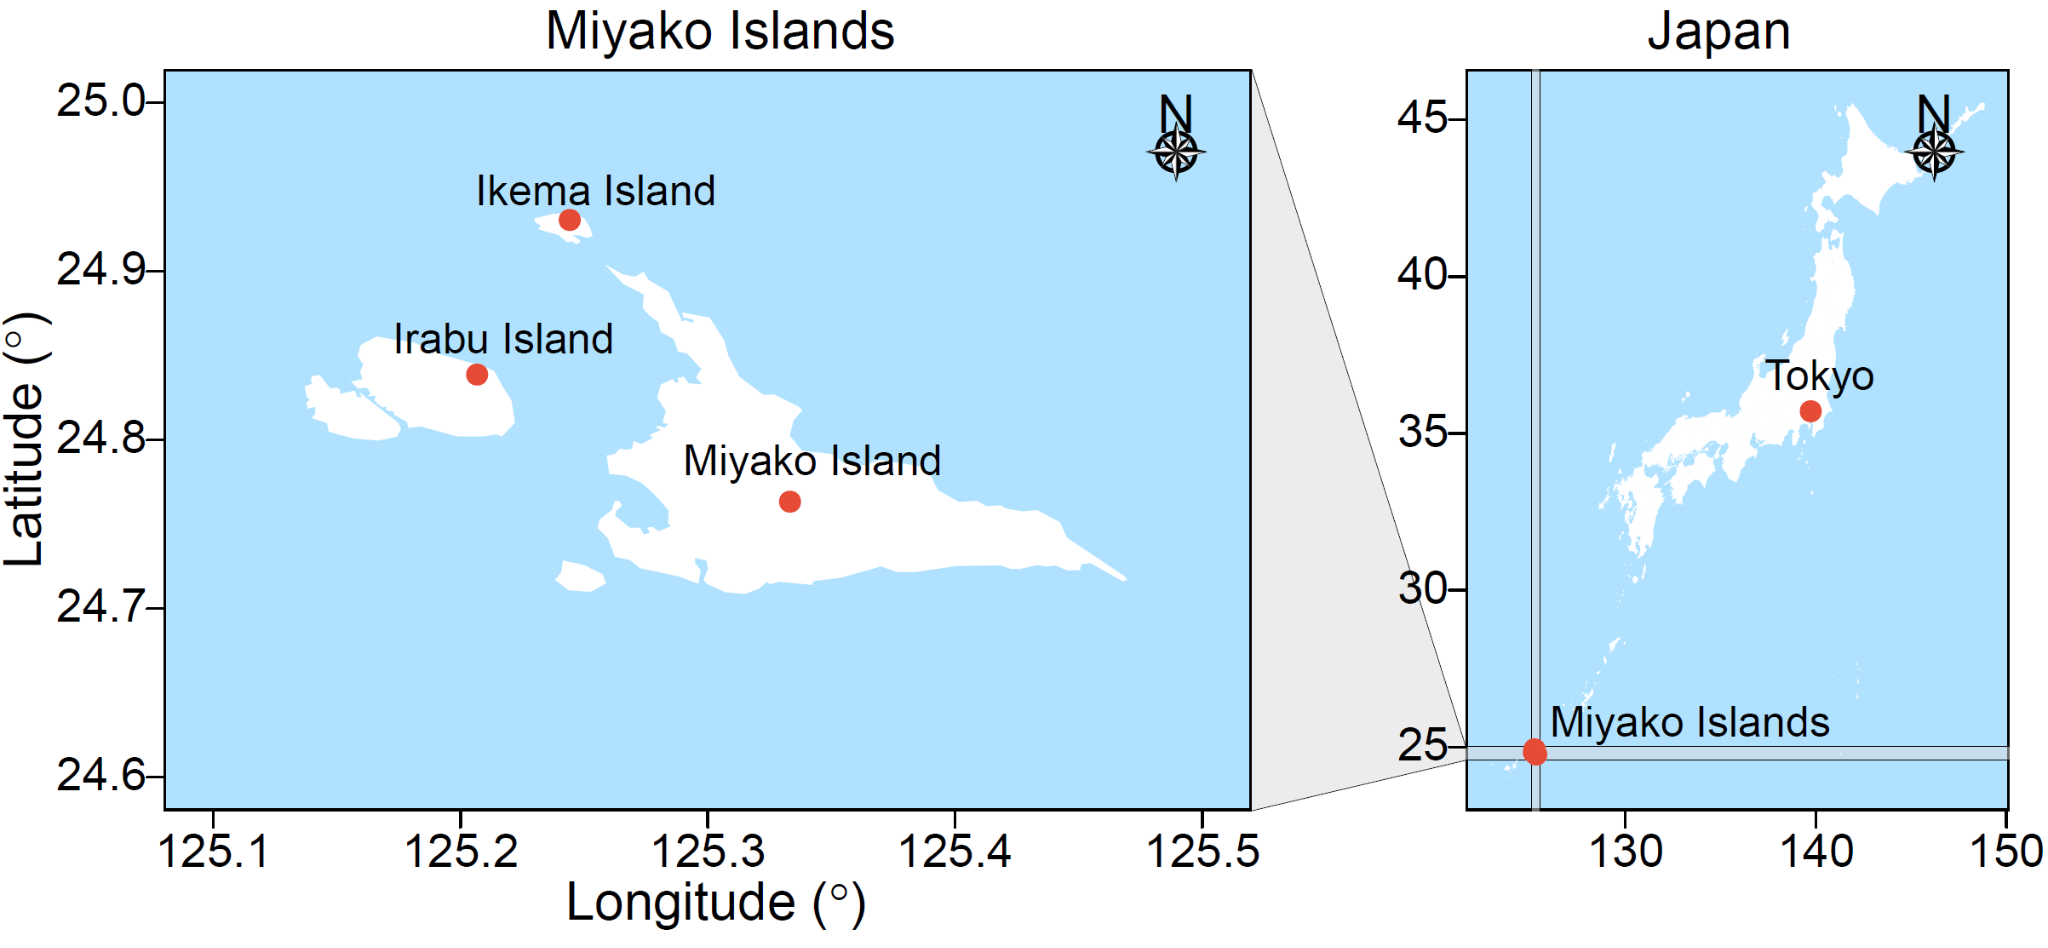
\includegraphics[width=\textwidth]{figures/a13ShinoharaHussainAmelot-img001.png}
\caption{\label{fig:shinohara:1}Location of the places where the Ikema dialect of Miyako Ryukyuan is spoken}
\end{figure}

Miyako Ryukyuan language has a wide range of word-initial and word-medial geminate consonants, but only the Ikema dialect has voiceless nasal consonants in its word-initial geminate inventory (\citealt{PellardHayashi2012}, \tabref{tab:shinohara:3}).

Our purpose is twofold: 

\begin{itemize}
  \item[(1)]  to assess the contrast between voiceless and voiced nasals in Ikema through phonetic investigation;
  \item[(2)]   to determine whether the voiceless nasals in Ikema can be classified among the previously identified similar sounds.
\end{itemize}

To achieve these goals, we have explored airflow and acoustic data from ten speakers of the Ikema dialect of Miyako Ryukyuan recorded in 2018. Additionally, we discuss the rarity of voiceless nasal geminates from the perspective of their evolutionary path.

\largerpage
The remaining parts of this section subsequently present Ikema phonology and phonetics from synchronic and diachronic perspectives and give an overview of the typology of voiceless nasals in a cross-linguistic context. \sectref{sec:shinohara:2} introduces relevant phonetic studies and our hypotheses for Ikema. \sectref{sec:shinohara:3} outlines the methods and procedures used in the current study. \sectref{sec:shinohara:4} presents the key findings of the study. Finally, \sectref{sec:shinohara:5} discusses our results and their implications for the typology of voiceless nasals.

\subsection{Ikema segmental phonology: synchrony}
\label{sec:shinohara:1.2}
\largerpage

Ikema features four basic vowel segments (\tabref{tab:shinohara:1}): /a/ (relatively open and central), /i/ (closed and front), /u/ (closed, back and rounded), and /I/ ([z̞] or [s]),\footnote{The diacritic mark in [z̞] indicates an open articulation. The voiceless phone appears when the vowel occurs between two voiceless obstruents.} a closed unrounded vowel where the main constriction is located at the alveolar ridge, creating weak frication noise in some cases and the second formant of which is found between [i] and [u] (\citealt{FujimotoShinohara2018}).\footnote{ In Miyako and southern Ryukyuans, a similar vowel has been described in different ways depending on the perspective. From an articulatory point of view, it has been labelled as an “apical” vowel /ɿ/ (e.g., \citealt{Sakiyama1963}), while from an auditory point of view, it has been described as a central vowel /ï/ (e.g., \citealt{Uchima1984}) or /i/ (e.g., \citealt{Hayashi2010}). A summary of the debate is found in \citet{OonoEtAl2000} and \citet{PellardHayashi2012}. \citet{FujimotoShinohara2018} investigated its place of articulation in Ikema using real-time magnetic resonance imaging and acoustic quality through formant frequencies. See \textcitetv{chapters/10_HugteEtAl} on the typology of fricative vowels.} This vowel occurs only after one of the homorganic consonants [s, ts, z] in Ikema. Additionally, two more vowel segments are used in a limited number of lexical items: /e/ (front mid-open) and /o/ (back mid-open), such as in /do/ ‘a sentence-final particle’ or /sjensjee/ [ɕeẽɕe:] ‘teacher,’ which is borrowed from Japanese.

\begin{table}
\begin{tabular}{llll}
\lsptoprule
Front  &     &   &   Back\\\midrule
Close  &   i & I & u   \\
       & (e) &   & (o) \\
Open   &     & a &     \\
\lspbottomrule
\end{tabular}
\caption{Ikema vowels}
\label{tab:shinohara:1}
\end{table}

The consonant segments occuring in Ikema are given in \tabref{tab:shinohara:2}.


\begin{table}
% \todo[inline]{I suggest dropping the voicing line with +-. Readers will know that /t/ is voiceless and that /d/ is voiced, even without explicit information to that effect\\
% I split the Approximant/Liquid category in two and put /w/ and /j/ in the approximant row and /ɾ/ in the liquid row. Maybe ``rhotic'' or ``tap'' could also be used as a label there.\\
% Maybe labio-velar can also be dropped as this level of precision for the approximant does not seem to contribute to the argument of the paper
% }
\small
\begin{tabularx}{\textwidth}{l QlQlll}
\lsptoprule
 & Labial (Labio-velar) & Alveolar & Alveolo- palatal & Palatal & Velar & Glottal\\
% \textbf{Voicing} &  \textbf{+} & \textbf{-      +} & \textbf{-     +} & \textbf{-      +} &    \textbf{+} & \textbf{-}\\
\midrule
Plosive & (p)\footnote{In the Nishihara variety of the Ikema dialect, singleton /p/ is used by some speakers; however, this is not the case in the Ikema variety. The Ikema dictionary based on the Nishihara variety includes words with /p/ \citep{NakamaEtAl2022}. Morphologically induced geminates may not all be included.},    b & t,      d &  &  & k,       ɡ & \\
& pp & tt,    dd &  &  & kk & \\
Fricative & f & s,     z & ɕ,    ʑ & ç &  & h\\
& ff,    vv & ss,   zz & ɕɕ &  &  & \\
Affricate &  & ts,   dz & tɕ,   dʑ &  &  & \\
&  & tts & ttɕ,  ddʑ &  &  & \\
Nasal & m & n &  &  &  & \\
& m̥m,  mm & n̥n,  nn &  &  &  & \\
Approximant & (w) &  &  & j &  & \\
Liquid      &     & ɾ&  &  &  & \\
\lspbottomrule
\end{tabularx}
\caption{Consonant inventory of Ikema}
\label{tab:shinohara:2}

\end{table}

\largerpage
In Ikema, segmental length (quantity) is contrastive, as it is in the majority of Japonic dialects (e.g., in Tokyo Japanese). Vowels contrast in length, except in underlyingly monomoraic words (see below). Consonants also exhibit length contrast manifested by gemination and represented in this chapter by double consonants.

Gemination occurs in certain consonants in word-initial and word-medial positions in Ikema. For example, the words /bada/ ‘gutter’ and /badda/ ‘side’ are differentiated solely by the length of the word-medial consonant. Some geminates are lexical and contrast with a singleton consonant, as in this example. Alternatively, a segment may become a geminate through a morphological operation (e.g., /dusI/ ‘friend’ alternates with /duss-a/ ‘friend.\textsc{top}’).

\largerpage
Here is a summary of the syllable types, analysed in standard moraic theory \citep{Hayes1989} for Ikema (\tabref{tab:shinohara:3}), except for some onset structures (see below). The syllable types in Ikema can be divided into two types: light and heavy syllables. Light syllables are composed of a short vowel with or without a simplex onset, cf. (a) in \tabref{tab:shinohara:3}. Heavy syllables manifest several subtypes. Heavy syllables can contain a long vowel (b) or a short vowel closed by a coda segment. Coda consonants are restricted to a nasal (c) and the first half of a geminate consonant (d). Heavy syllables can also start with a geminate consonant (e) or a moraic nasal followed by an obstruent (f). In structure (f), only homorganic consonant sequences are allowed. A nasal consonant can also form a heavy syllable without a nucleus vowel (g), although only a few lexical items seem to involve this structure.\footnote{The Ikema dictionary \citep{NakamaEtAl2022} records two homophonous verbs, /n̥n/, which mean ‘to ladle’ and ‘to step on.’ The sound /n̥n/ is also present in some compound verbs, such as [n̥nta:] ‘to trample.’ As this dictionary is based on a single speaker, it is not possible to determine whether this structure represents a phonologically regular pattern.}

\begin{table}

\begin{tabularx}{\textwidth}{lXl}
\lsptoprule
Light syllable type (1 mora) & (C)V      &  (a) [sa.ba] ‘shark’\\
\tablevspace
Heavy syllable types (2 moras) & (C)V:   &  (b) [na:] ‘name’  \\
                                        &  (C)VN  &  (c) [in] ‘dog’        \\
                                        &  (C)VC  &  (d) [maf.fa] ‘pillow’ \\
                                        &  CCV    &  (e) [tta] ‘tongue’    \\
                                        &  NCV    &  (f) [nta] ‘soil’      \\
                                        &N:       &  (g) [n:] ‘potato’ \\
\lspbottomrule
\end{tabularx}
\caption{Surface syllable types of Ikema. C represents a consonant, V = a vowel, N = a moraic nasal, N: = a syllabic nasal. A dot marks the syllable boundary}
\label{tab:shinohara:3}
\end{table}

In the moraic framework, the onset consonants are considered weightless. A word-medial geminate is treated as a single segment that affiliates with the moraic coda position of one syllable and simultaneously with the onset position of the following syllable. Word-initial geminate consonants are less common cross-linguistically than those found in the word-medial position (\citealt{Dmitrieva2012,HamzahEtAl2020,Kraehenmann2001,Muller2003,Thurgood1993}). The occurrence of geminates in the syllable onset positions poses a challenge to this theory. However, in some languages, onset consonants play a role in prosodic organisations such as stress or tone assignment, which indicates that they can bear prosodic weight (\citealt{Davis1999,Gordon2004,Topintzi2008,ShinoharaFujimoto2011}). We also adopt the perspective that moraic segments can in principle appear in a syllable onset position.

Phonological evidence supports the moraicity of the initial geminates in Ikema. Monomoraic words always surface with two moras due to the bimoraic word minimality constraint. For example, /na/ ‘name’ and /ti/ ‘hand’ surface as [naː] and [tiː], respectively. This constraint is observed in many Ryukyuan dialects, including Ikema (\citealt{Shimoji2010,PellardHayashi2012}). However, vowel lengthening does not occur in words such as /nna/ ‘spiral shell’ or /tta/ ‘tongue’. This indicates that the initial consonant is moraic, and so the overall output length of these words already satisfies the bimoraic word minimality constraint. The vowel does not lengthen in a monosyllabic word starting with a voiceless nasal (/n̥na/ [n̥na] ‘rope’) either, which shows the moraicity of this consonant.

\largerpage
Previous phonological analyses of Ikema have consistently considered the first half of the [m̥m] and [n̥n] sequences as moraic. However, these sequences have been treated as sequences of two nasals, as analysed in linear phonological models, rather than as single geminate consonants (\citealt{Hirayama1983,Uchima1984,Hayashi2007,Hayashi2010,IgarashiEtAl2011,Takubo2021,NakamaEtAl2022}). In contrast, \citet{ShinoharaFujimoto2018} have recognised these units as “half voiceless nasal geminates”. In this study, we refer to the sounds in question as “voiceless nasal geminates”. However, we continue to use the conventional and phonetically realistic transcription, i.e., a sequence of a devoiced nasal element followed by a plain nasal. “Voiceless nasals”, in turn, are used as a general term covering any voiceless nasal segments in any language regardless of their length.


\begin{table}[b]
\begin{tabularx}{.8\textwidth}{XXl}
\lsptoprule
 & Word-initial position & Word-medial position\\
 \midrule
Voiceless & \it{tta} ‘tongue’    & \it{uttu} ‘brother’                         \\
                   & \it{ttɕutsI} ‘cicada’&                  \it{attɕa} ‘geta clogs’    \\
                   & \it{ffa} ‘child’     &                  \it{maffa} ‘pillow’        \\
                   & \it{ssa} ‘grass’     &                  \it{uss-a} ‘cow.\textsc{top}’       \\
                   & \it{m̥mu} ‘cloud’    &                  --                    \\
                   & \it{n̥na} ‘rope’     &                  --\\
\tablevspace
Voiced & --                   & \it{badda} ‘side’           \\
                & --                   & \it{tuddʑ-a} ‘wife.\textsc{top}’     \\
                & \it{vva} ‘you’            & \it{avva} ‘oil’             \\
                & \it{zza} ‘father’         &     --                 \\
                & \it{mma} ‘mother’         & \it{haamma} ‘grandmother’   \\
                & \it{nna} ‘spiral shell’   & \it{kannai} ‘thunder’\\
\lspbottomrule
\end{tabularx}
\caption{Voicing contrast in Ikema geminate consonants. A symbol “--" indicates a systematic gap}
\label{tab:shinohara:4}
\end{table}


The particularity of Ikema phonology lies in the richness of the subsystem of geminate consonants (a summary of which is provided in \tabref{tab:shinohara:4}). Unlike other Japonic languages such as Okinawa or Yaeyama Ryukyuan, which have only voiceless geminate consonants, Ikema displays a variety of voiced and voiceless geminates. However, there are also numerous gaps in terms of both the types of segments and the types of positions in the distribution of geminates. For example, voiceless nasal geminates occur only in the morpheme-initial position. \citet{Hayashi2010} noted that, among the obstruents, /tt, tts, kk, ff, ss, vv, zz/ can occur as initial geminates. Additionally, certain segments such as /m̥ , n̥ , p, v/ do not appear as singletons in any position and only occur as (or as part of) geminates. On the other hand, singletons /b/ and /ɡ/ lack their respective geminate counterparts. Geminates /pp, kk/ are rare (e.g., /bappai/ ‘mistake in calculation’ and /kkunutsI/ {\textasciitilde} /kukunutsI/ ‘nine’).


Ikema is a language that uses a three-way pitch-accent system, where lexical items are specified for one of the three abstract categories: A, B or C type. This terminology is used in the historical linguistics of Japonic languages, as described in \citeauthor{IgarashiEtAl2011} (\citeyear{IgarashiEtAl2011} et seq.). According to Igarashi et al. (2011 et seq.), bi- and trimoraic words in isolation neutralise pitch accents for A and B types. In trimoraic words, the first mora of all types can be either low- (L) or high- (H) toned. The pitch patterns for the two-mora words are HL (A and B types), LH or HH (C type), while those for the three-mora words are LHL or HHL (A and B types), and LHH or HHH (C type). \citet{IgarashiEtAl2018} discovered that a full distinction of the accent types is conditioned by the number of prosodic words in an utterance. Nevertheless, there are still numerous unresolved issues in the description of the pitch-accent system. As they are not directly relevant for the purposes of this chapter, we do not discuss them further.

\subsection{Ikema segmental phonology: diachrony of voiceless nasal geminates}
\label{sec:shinohara:1.3}
By comparing cognate words across different dialects, it is possible to trace the phonetic changes which have led to the occurrence of voiceless nasal geminates. We list some synchronic forms of three words with voiceless nasal geminates drawn from \citet{Kibe2012} in \tabref{tab:shinohara:5}. One key characteristic of the voiceless nasals is that they correspond to a voiceless obstruent accompanied by an element with frication noise in cognate words. This element can be a fricative consonant or the vowel represented by /I/ in our transcription. This vowel corresponds to /ɿ/ or /ï/ in \tabref{tab:shinohara:5}. It occurs in wider consonantal contexts and preserves more frication noise in some other Miyako dialects, such as Karimata, Hirara or Bora among others, than in /I/ in Ikema \citep{Kibe2012}. \citet[50]{PellardHayashi2012} posited that all initial geminate plosives in Miyako Ryukyuan have developed out of vowel elision. Among other things, they suggested that the initial nasal sequences found in Ikema likely result from the syncope of a high vowel (p. 47). 


\begin{table}
\begin{tabularx}{\textwidth}{lXlXlXl}
\lsptoprule
 & Ikema & Yonaha & Kugai & Kurima & Bora & Proto Miyako\\
 \midrule
‘cloud’ & m̥mu & fʊm & fumu & fumu & fumu & *fumu\\
‘yesterday’ & n̥nu & kˢɿ̥nʊ & ksïnu & ʦïno & kˢɿnuː & *kɿnuː\\
‘horn’ & n̥nu & ʦɿnʊ & ʦïnu & ʦïnu & ʦɿnu & *tsɿnu\\
\lspbottomrule
\end{tabularx}
\caption{Cognate forms in Miyako Ryukyuan dialects. Based on data from \citet{Kibe2012}}
\label{tab:shinohara:5}
\end{table}

Phonetic explanations have been provided for the development of voiceless nasals in other languages, and they can be applied also to the case of Ikema. \citet{Ohala1975} and \citet{OhalaOhala1993} observed that voiceless nasals in Burmese have their origin in a sequence of [s] followed by a nasal stop, as depicted in the orthography of corresponding Tibetan words. \citet{BarryKunzel1978} explicated the gradient nature of progressive partial devoicing of sonorants after a voiceless obstruent in German and English, in words like \textit{small}. They argued that the nasal component is typically partially devoiced due to asynchrony in velum opening, a shift of oral constriction place and voicing coordination. The present study hypothesises that a gradient phonetic assimilation may result in a phonological change, particularly when incited by a shift in the prosodic structure. In cases where only one consonant slot remains in the prosodic template, one possible solution for segmental reduction is the use of a coalesced form to fill the slot. In the case of Ikema, the preservation of this consonant slot as moraic after vowel syncope may have saved the prosodic shape of a word intact even after a segmental change. As the pitch-accent location is determined by the mora count from the beginning of the word (\citealt{IgarashiEtAl2011} et seq.), the loss of the first mora would have altered the prosodic shape of the word.

\citet{OhalaBusà1995} argued for the perceptual similarity between vowels adjacent to fricatives and to nasals from an aerodynamic perspective. This similarity has induced nasal loss in fricative contexts in sound changes in many unrelated languages, as seen in German \textit{Gans} to English \textit{goose} or Latin \textit{mensis} to Italian \textit{mese}. Less frequently, the similarity has also induced spontaneous nasalisation of vowels adjacent to a fricative or apparition of a nasal consonant such as in Sanskrit \textit{sarpa} ‘snake’ > Hindi /sãp/, or Latin \textit{bonaça}. bon- ‘good’ > Spanish \textit{bonanza} [bonansa]. However, segments whose production requires high airflows, such as affricates or aspirated stops, do not promote nasal loss (\citealt{OhalaBusà1995}: 22). According to Ohala and Busà’s theory, the fricative in Ikema’s sequence, such as [fumu], could have resulted in a nasalised vowel as in inexistent *[\~umu]. But instead, the syllable is deleted leaving the voiceless and fricative features of the initial consonant. This sound change might have been incited by the already existing voicing contrast in initial geminates in the language (e.g., /ffa/ ‘child’ vs. /vva/ ‘you’ in \tabref{tab:shinohara:4}). Indeed, the latter type of initial obstruent geminates are widespread across Miyako Ryukayun dialects, but Ikema is the only dialect which has developed voiceless nasals. \footnote{\citet{Uchima1984} observed that voiceless bilabial and alveolar nasals are present in Karimata Miyako Ryukyuan and Kabira Yaeyama Ryukyuan. In Kabira Yaeyama Ryukyuan, voiceless singleton nasals occur in the context of sonorant devoicing, where a sonorant onset is devoiced when following a devoiced vowel \citep{Kajiku1984}. This phenomenon is common across many Yaeyama Ryukyuan dialects, and the resulting voiceless nasals are not contrastive. With regard to the Karimata dialect, the data collected in 2011 by \citet{Kibe2012} and the dialect study by \citet{KinuhataHayashi2014} do not provide evidence for voiceless nasal sounds.} Therefore, we assume that the voiceless nasals developed later than the initial geminate obstruents.

\subsection{Typological comparanda for voiceless nasals}
\label{sec:shinohara:1.4}

\sloppy
Cross-linguistically, contrastive voiceless nasals are rare, although partially or entirely devoiced nasals may occur as allophones of nasals. In some languages, nasal stops become partially devoiced when adjacent to a voiceless obstruent, which results in voiceless frication noise through the nasal cavity. \citet{Gimson1980} provides the following examples of devoiced nasals in English: \textit{topmost} [tɒpⁿm̥əʊst], \textit{chutney} [ʧʌtⁿn̥ɪ]. \citet{Dell1973} gives the following sequences in French as examples of non-distinctive voiceless sonorants: \textit{cette natte} [sɛtⁿn̥at] ‘this plait’, \textit{cette masse} [sɛtⁿm̥as] ‘this volume’, \textit{vous semez} [vu sm̥e] ‘you sow’. While voiced nasal stops are sonorants, the devoiced ones are phonetically fricatives, like any other sonorant consonants which become fricative sounds when devoiced. For instance, the devoiced [l] is a voiceless lateral fricative [ɬ].

\citet{OhalaOhala1993} characterised voiceless nasal sounds as non-optimal speech sounds because the nasal cavity is not suitable for intense noise generation. \citet{Ohala1975} noted that the place distinction for voiceless nasals would not be made because noise spectra of voiceless nasals are similar for any of the places of articulation. Therefore, the place distinction is only possible for the voiced portion of a voiceless nasal segment. He also predicted that voiceless nasals should be prone to deletion because of their low-intensity noise.

\fussy\largerpage
According to the geospatial distribution of the world’s languages in PHOIBLE (\citealt{MoranMcCloy2019}), which is the largest database of phonemic inventories, voiced nasal /m n/ are widely attested across languages (/m/ 96\%, /n/ 78\%). However, their voiceless counterparts /m̥ n̥/ are found only in 2\% of the world’s languages. The UCLA Phonological Segment Inventory Database (UPSID) (\citealt{MaddiesonPrecoda1990}) lists 18 languages (4\%) among the 451 languages of the world that have voiceless nasals at least at one place of articulation. Non-contras\-tive voiceless nasals are not included in UPSID. A similar result is obtained in the Lyon-Albuquerque Phonological Systems Database (LAPSyD) (\citealt{MaddiesonEtAl2016}). LAPSyD lists 31 (4.5\%) out of 683 languages with at least one voiceless nasal and 19 languages (2.8\%) having both bilabial and alveolar voiceless nasals. None of the aforementioned databases lists any Ryukyuan languages.

\begin{sloppypar}
The Ikema language exhibits a unique feature in that its voiceless nasals only occur as word-initial geminates, a phenomenon not reported for any other known language to the best of our knowledge. Word-initial voiceless nasal geminates are expected to be very rare, because they present a combination of rare factors. First, voiceless nasals in themselves are rare, as previously illustrated. Additionally, geminates are rarer than singletons, as all languages possess singleton consonants but only some possess geminate consonants. Finally, initial geminates are typologically rarer than intervocalic geminates, as noted in previous studies (\citealt{Thurgood1993,Dmitrieva2012}). Of all segmental types, voiceless plosives and nasal stops are the most common segments for gemination in word-medial position, according to studies by \citet{Jaeger1978}, \citet{Kirchner2001}, \citet{Podesva2002} and \citet{Maddieson2008}. In word-initial position, nasal geminates have been found in 22 languages out of 28 surveyed for initial geminates (\citealt{Muller2001}: Appendix), although none of these languages has voicing contrasts in nasal geminates.
\end{sloppypar}

\section{Previous studies on voiceless nasals and hypotheses for Ikema}
\label{sec:shinohara:2}
This section begins by reviewing aerodynamic studies of voiceless nasals in other languages \sectref{sec:shinohara:2.1}. We then show that timing patterns of voicing are essential for the characterisation of voiceless nasals. Because of this, we provide additional details on the durational correlates of voiceless nasals in \sectref{sec:shinohara:2.2}. In \sectref{sec:shinohara:2.3}, we review non-temporal acoustic studies on voiceless nasals and summarise our hypotheses based on the previous studies.

\subsection{Aerodynamic patterns of voiceless nasals}\label{sec:shinohara:2.1}
Except for Ikema, no voiceless nasal geminates have been reported. Therefore, the following description pertains to voiceless nasals as singletons. Contrastive voiceless nasals of Tibeto-Burman languages and Tibetan have been instrumentally studied (\citealt{Dantsuji1984,Dantsuji1986,BhaskararaoLadefoged1991}). Based on their investigations of Burmese, Mizo and Angami, \citet{BhaskararaoLadefoged1991} classified voiceless nasals into two types: “Burmese” and “Angami” (\tabref{tab:shinohara:6}).\footnote{ Their study included recording corpora of Burmese (four minimal pairs with four distinct places of articulations differing in voicing by six speakers), Mizo (three minimal pairs with three places of articulations with three speakers) and Angami (three minimal pairs with three places of articulations with nine speakers) all uttered within frame sentences.}

\begin{table}
\begin{tabularx}{\textwidth}{lQQQ}
\lsptoprule
{Types} & {Acoustic pattern} & {Airflow pattern} & {Languages}\\
\midrule
{Burmese} & {Voiceless frication noise followed by a voiced nasal} & {Nasal airflow without oral airflow} & {Burmese (Myanmar)}\newline {Mizo (Northeast India)}\\
\tablevspace
{Angami}  & {Post-aspirated; mostly voiceless during their release interval}  & {Simultaneous oral and nasal flows at the release phase} & {Angami (Northeast India)}\newline {Xumi (Southwest China)}\newline {Tibetan (Southern China)}\\
\lspbottomrule
\end{tabularx}
\caption{\label{tab:shinohara:6} A summary of the two different types of voiceless nasals, after \citet{BhaskararaoLadefoged1991}}
\end{table}

The best-known type, the Burmese type, consists of two acoustic/articulatory events: (a) voiceless frication noise followed by (b) a voiced nasal before a release. While the presence of the voiceless frication is necessary to establish a contrast with regular voiced nasal stops, a period of voicing is also needed for the identification of the place of articulation in voiceless nasals. Without a voiced release, place cues may be too ambiguous in nasals (as pointed out by \citealt{Ohala1975}; see also \citealt{KurowskiBlumstein1993} for place cues in nasal consonants). Based on perception experiments, \citet{Dantsuji1986} claimed that the bilabial, alveolar and velar places of voiceless nasals in Burmese are identified in the portion of voiced murmur following the voiceless part of the voiceless nasal segments.

The voiceless nasals of another type, represented by Angami, are entirely voiceless throughout their release interval. \citet{BlankenshipEtAl1993} reported that there is a nasalised aspiration period between the release of oral closure and the onset of vocal fold vibration for the following vowel, where both oral and nasal airflows are observed. These facts have led to the coining of the term “aspirated voiceless nasals” for this type of voiceless nasal (\citealt{LadefogedMaddieson1996}). \citet{ChirkovaEtAl2019} identified two other languages of this type (see below). \citet{bell2021northern} reported that Northern Welsh also has a voiceless nasal of this type. We examine below some additional details of previous findings that are relevant to our study.

\citet{ChirkovaEtAl2019} conducted a study on voiceless nasals in three Tibeto-Burman languages (Xumi, (Kham-)Tibetan and Burmese), using audio, electroglottography (EGG), oral and nasal airflows and video recording of the lips. This study showed two distinct nasal and oral airflow timing patterns. Xumi (Tibeto-Burman language of Southwest China) has /m̥/ and /n̥/ as distinct voiceless nasal consonants. They are characterised by simultaneous oral and nasal flows. This indicates that the latter part of the oral constriction is loosened, resulting in a nasalised voiceless glottal fricative. Tibetan showed similar airflow patterns as Xumi and so it also belongs to the Angami type. In contrast, Burmese has a different pattern in which the voiced part following the voiceless part has no oral flow, which results in a regular nasal stop. While place cues may not be found within nasals, visual cues and formant transitions during the following vowel may play a role in cueing place in Xumi voiceless nasals, as suggested by \citet{ChirkovaEtAl2019}, and also by \citet{GogoiWayland2018} for the Angami case. 

Based on the phonological descriptions and previous acoustic studies of voiceless nasals in Ikema (\citealt{Hirayama1983,Uchima1984,Hayashi2007,Hayashi2010,IgarashiEtAl2011,Takubo2021,NakamaEtAl2022,ShinoharaFujimoto2018}), it is expected that Ikema belongs to the Burmese type, with its release phase preceded by a voiced interval. The study of the airflow patterns of voiceless nasals in Ikema provides another test for this assumption.

\subsection{Durational correlates of Ikema voiceless nasal geminates}\label{sec:shinohara:2.2}
Here we examine the durational patterns of voiceless nasal geminates, both as a whole and in terms of the proportions of their voiceless and voiced parts. Previous acoustic study of Ikema, described in more detail below, has shown a smaller voiceless proportion in durational patterns as compared to other languages (\citealt{ShinoharaFujimoto2018}). \citet[111]{LadefogedMaddieson1996} noted that voiceless nasals are generally longer than voiced ones. Regarding the proportion of voiceless and voiced parts, \citet{ChirkovaEtAl2019} measured the duration of voiceless nasal segments both in frame sentences and in isolation. Based on the electroglottography data on bilabial and alveolar nasals, they found that the voiced portion of voiceless nasal segments in Burmese is 33\%. \citet[2]{Dantsuji1986}, whose test words appear to have been uttered in isolation, reported that the voiced portion formed the last 25--29\% of voiceless nasals and is much shorter than that of the ordinary voiced nasals in Burmese.

In Ikema, \citet{ShinoharaFujimoto2018} examined acoustic recordings from five speakers in the Nishihara area of Miyako Island. They found that in words with voiceless nasals uttered in isolation, the voiced proportion is 83.5\%.

In many languages, the contrast in phonological length between singleton and geminate consonants is primarily manifested by their phonetic duration (\citealt{LahiriHankamer1988}, among others). Acoustic confirmation of this for Ikema fricative and nasal consonants with phonological length contrast was obtained by \citet{ShinoharaFujimoto2018}. The duration of [nn] in /nna/ ‘spiral shell’ was 183~ms, which is significantly different from that of [n] in /nada/ ‘tears’ of 79~ms.

The same study also examined the timing units of Ikema words. For words with varying numbers of moras and syllables, duration has been found to correlate better with the number of moras than with the number of syllables. This result is similar to what has been found in Tokyo Japanese, where word duration is controlled by mora count (\citealt{SagisakaTohkura1984}). Therefore, one would expect that a nasal geminate consonant would have a duration approximately equivalent to that of a light syllable, all other conditions being equal. However, the duration of words with a geminate, as measured in the acoustic signal (e.g., the entire duration of /nna/ ‘spiral shell’ or /n̥na/ ‘rope’), was significantly shorter than that of other bimoraic words (e.g., /nada/ ‘tears’). Additionally, contrary to the hypothesis put forward by \citet{LadefogedMaddieson1996}, voiceless nasal geminates have not been found to be longer than the voiced ones (see \figref{fig:shinohara:2}).




\begin{figure}
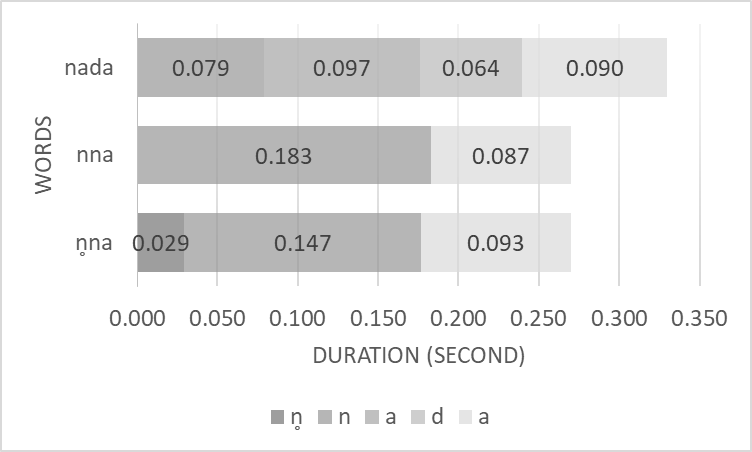
\includegraphics[width=\textwidth]{figures/a13ShinoharaHussainAmelot-img002.png}
\caption{\label{fig:shinohara:2}Segmental durations in /nada/ ‘tears’, /nna/ ‘spiral shell’, and /n̥na/ ‘rope’ measured in acoustic signals (in seconds) for five speakers, eleven tokens per item, by \citet[264]{ShinoharaFujimoto2018}, Figure 15.12)}
\end{figure}

We hypothesise that the findings of the current study would replicate the previously observed longer duration of voiceless geminate consonants compared to singleton onset consonants in Ikema. Additionally, we expect that the rate of voicing for voiceless nasals in Ikema may differ from the cross-linguistically observed pattern in that its proportion is greater.

\subsection{Non-temporal acoustic correlates of voiceless nasals}\label{sec:shinohara:2.3}
\citet{Ford2016} and \citet{FordEtAl2022} conducted acoustic investigations of voiceless nasals in six speakers from the Ikema Island. They have identified a significant distinction in the periodicity of nasal sounds between voiceless and phonologically voiced nasals. Specifically, they found that voiceless nasals exhibit lower Cepstral Peak Prominence (CPP) values, which indicates the non-periodic nature of these sounds (see \citealt{HillenbrandEtAl1994} for CPP). Likewise, the study by \citet{ShinoharaFujimoto2018}, mentioned in \sectref{sec:shinohara:2.2}, reported the presence of a short voiceless frication noise with a formant structure similar to the subsequent voiced nasal segments in words such as /m̥mu/ ‘cloud’ and /n̥na/ ‘rope’. However, the words containing voiced nasal consonants, such as /maffa/ ‘pillow’ and /nna/ ‘spiral shell’, did not exhibit a discernible formant structure preceding the voiced nasal on the spectrogram. The observed formant structures during the frication period suggest that the voiceless portions are articulated with an oral constriction similar to the subsequent nasal segments. These findings confirm the acoustic distinction in terms of periodicity between voiceless and voiced nasals in Ikema.

The non-temporal aspect of our present acoustic study focuses on the acoustic properties of the onset of the following vowel. Acoustic cues that efficiently signal voiceless nasals in other languages include fundamental frequency (f0) and several breathiness measures. F0 has been extensively investigated as a significant acoustic correlate for distinguishing voicing and/or aspiration in different languages (see \citealt{Hombert1978}; \citealt{Hussain2021}, and references therein). Studies have demonstrated that voiceless nasals incur higher f0 onsets, as compared to voiced nasals (\citealt{Maddieson1984}; \citealt{Kirby2021}). \citet{Maddieson1984} has discovered that f0 increases following voiceless nasals in Burmese. Similarly, based on the examination of a non-tonal Eastern Khmu language spoken in Laos, \citet{Kirby2021} noted that voiceless sonorants (referred to as “continuants” in his terminology) incur even more pronounced f0 perturbation at the onset of the following vowel compared to voiceless obstruents. Therefore, we expect that voiceless nasals might have a higher f0 at the onset of the following vowel in comparison to voiced ones.

\citet{GogoiEtAl2018} investigated voiceless nasals in Mizo, a Tibeto-Burman language spoken in Northeast India. \citet{BhaskararaoLadefoged1991} had previously observed that Mizo has an airflow pattern similar to Burmese. Gogoi et al.’s study focused on measuring breathiness at the onset of the following vowel caused by voiceless nasal articulation in Mizo. They used H1-H2, the difference between the first and the second harmonics, which is a widely used measure of breathiness of the voice quality \citep{Johnson1997}. The findings of \citet{GogoiEtAl2018} have shown that H1-H2 is more similar to breathy voice at the onset of a vowel following a voiceless nasal than when following a voiced nasal stop. This acoustic difference may serve as a cue also for the voicing contrast in nasals.

Based on the previous studies, the acoustic measures mentioned above may indicate voicing differences in nasals. However, in the case of Ikema, a nasal has a long voiced interval after the voiceless period. Therefore, there may be no differences in f0 and H1-H2 at the onsets of the vowels following voiceless and voiced nasals. Considering the typology of voiceless nasals, a completely voiceless nasal without any voicing gesture is not plausible from aerodynamic and articulatory perspectives. Therefore, depending on the proportion of voiced part after the voiceless one, the impact from voiceless nasals on f0 and other acoustic values at the following vowel onset may be variable. We aim to determine what the case of Ikema is.

However, we also need to consider certain artefacts in our experiments. The number of Ikema words involving voiceless nasals is limited, which makes it impossible to establish a perfect paradigm. In addition to the difference in voicing, three other factors potentially contribute to the elevation of f0 in our data. First, it is well-known that close vowels have higher f0 as compared to open vowels (\citealt{WhalenLevitt1995}). Second, recent studies have reported higher f0 at the onset of the vowel after geminate consonants of certain segments, as opposed to singletons. \citet{HamzahEtAl2020} have demonstrated that voiceless plosive geminates effectively raise f0 in Kelantan Malay along with nasals and laterals. \citet{BurroniEtAl2021} have also reported that initial geminate consonants are associated with higher f0 values during the following vowel in Pattani Malay, Salentino and Dunan. Finally, a high tone assigned from the lexical pitch-accent may also impact f0 at the vowel onset (this was not entirely controlled in our study). Therefore, follow-up evaluations were conducted to determine whether vowel quality, geminacy or pitch-accent might affect f0 values instead of voicing.

Our hypotheses on the aerodynamic and acoustic measurements are summa\-rised as follows.

\begin{enumerate}
\item The aerodynamic patterns of Ikema’s voiceless nasal will either follow one or the other of the two cross-linguistically recognised types – the Burmese or the Angami type – or represent a new type.
\item Since phonological descriptions and previous acoustic studies have indicated that the voiceless nasals of Ikema are composed of a voiceless interval followed by a relatively long voiced interval, the voicing rate in these sounds is likely to be greater than reported for other languages.
\item The voicing state of the nasal consonant influences f0 and H1-H2 values at the onset of the subsequent vowel. Nevertheless, the voiceless nasals in Ikema may not exhibit the expected effects due to the extended duration of their voiced part. In our (follow-up) analyses, the following factors are expected to exhibit elevated f0 values: the vowel /u/ (in comparison to  \mbox{/a/}), a vowel following a geminate consonant (as compared to a singleton consonant), and a vowel assigned a high tone through lexical pitch-accent (in contrast to the one with an expected low tone).
\end{enumerate}

\section{Methods}
\label{sec:shinohara:3}
To investigate the voiceless nasal geminates of Ikema in comparison with voiced singletons and voiced geminate nasals, we have employed both aerodynamic and acoustic data. We have examined the patterns of oral and nasal airflows. The acoustic analysis encompasses consonant duration and selected non-temporal measurements, namely f0 and H1*-H2*, at the onset of the following vowel. H1*-H2* is a corrected measure of H1-H2, with asterisks indicating that the corrections were made for the boosting effects of formant frequencies and bandwidths (\citealt{IseliEtAl2007}, see \citealt{StevensHanson1995} for the corrected measures). If higher f0 or higher H1*-H2* values are observed, it may indicate the voicelessness of the nasals. We have compared these values between voiceless and voiced nasals in our test words. Furthermore, we have calculated the durational proportions of the voiceless and voiced parts within voiceless nasal geminates.

\subsection{Speakers}
\label{sec:shinohara:3.1}
Ten Ikema speakers participated in the study, all of whom were born and raised on Ikema Island. Three male participants were born between 1952 and 1959 (with a mean age of 61.7 years at the time of recording in 2018), while seven female participants were born between 1932 and 1952 (with a mean age of 75.6 years). One male and two female participants had left Ikema Island during adulthood to study and work in Naha, Okinawa, or Kagoshima, before returning to live on Ikema Island or in Hirara on Miyako Island in their twenties. Those who reside on Miyako Island commute to Ikema Island for work and maintain regular contact with other Ikema speakers. The remaining participants have lived their entire lives on Ikema Island. In addition to speaking Ikema Miyako, all participants are bilingual in Japanese, as is typical of all current Ryukyuan speakers.

\subsection{Test words}
\label{sec:shinohara:3.2}
A collection of 13 test words was initially obtained from two sources, namely, \citet{Kibe2012} and the word list developed for an Ikema dictionary (Hiroyuki Nakama, p.c., August 2018). The selected words were either minimal pairs or quasi-minimal pairs (as listed in \tabref{tab:shinohara:7}). The list included four words with initial voiceless nasal geminates (two of which were segmentally homophonous), three words with initial voiced nasal geminates, two words with initial voiced singleton nasals, two words with medial singleton nasals and two words with medial geminate nasals. Three tokens of each test word were recorded from each speaker (however, see below for variation). The aerodynamic analyses included the following subset of comparable test words: \textit{maffa, mma, hmmu, naa, nna, hnna} (the voiceless part in /m̥m/ and /n̥n/ is represented as \textit{hm} or \textit{hn}, respectively, in word forms in figures, tables and elsewhere). The main acoustic analysis included the same six words. Two more words, /n̥nu/ ‘yesterday’; ‘horn’ were used in the additional (follow-up) analyses of f0. The durational analyses were based on 12 words.


\begin{sidewaystable}
% \todo[inline]{check new headers}
\small
\begin{tabularx}{\textwidth}{llllrrYYY}
\lsptoprule
   &
   &
   &
   &
   &
\multicolumn{4}{c}{Token number in analyses}\\
\cmidrule{6-9}
{Word}   &
{Gloss} &
{Accent}&
{Label} &
{Moras} &
{Airflow } &
{Main non-temporal } &
{Additional \mbox{non-temporal}} &
{Durational }\\
\midrule
maffa & pillow & B &  & 3 & 30 & 28 &  & 30\\
na [na:] & name & B & \textit{naa} & 2 & 36 & 36 & 36 & 30\\
mma & mother & C &  & 2 & 30 & 30 & 30 & 30\\
nna & spiral shell & B &  & 2 & 32 & 32 & 32 & 30\\
n̥na & rope & B & \textit{hnna/}\newline \textit{hnnaa} & 2 & 23 & 23 & 23 & 4\\
*nnu & straw rain cape & B &  & 2 &  &  &  & \\
n̥nu & yesterday & C & \textit{hnnu} & 2 &  &  & 30 & 30\\
n̥nu & horn & B & \textit{hnnu} & 2 &  &  & 29 & 29\\
m̥mu & cloud & B & \textit{hmmu} & 2 & 27 & 27 & 27 & 27\\
kama & over there & ? &  & 2 &  &  &  & 28\\
ana & hole & ? &  & 2 &  &  &  & 27\\
hammai & food & ? &  & 4 &  &  &  & 30\\
kannai & thunder & ? &  & 4 &  &  &  & 29\\
\midrule
{Total token number} &  &  &  &  & 178 & 176 & 207 & 324\\
\lspbottomrule
\end{tabularx}
\caption{Test words, their characteristics and token numbers of each experiment. *nnu is a word not recognised by our speakers and is excluded from the analysis}
\label{tab:shinohara:7}
\end{sidewaystable}

Some segmental variation was noted across speakers. This may be attributed to regional differences, since the test words were mainly collected from the glossary of the Nishihara area on the main Miyako Island. Among the 13 words, one with an initial voiced nasal geminate /nnu/ ‘straw rain cape’ was not recognised by the speakers. This has made it impossible to compare /nnu/ with its voiceless counterpart /n̥nu/. As a result, the two voiceless items /n̥nu/ ‘yesterday; rope’ were excluded from the voicing comparisons. Two speakers produced the voiceless word /n̥na/ ‘rope’ as [naa], and one speaker did so twice out of the three tokens. This case was treated as having no voiceless interval. The same word was often produced with a long vowel ([n̥naa]) by six speakers. These tokens were excluded from the durational analyses but included in the other analyses. One speaker did not produce /m̥mu/ ‘cloud’. F0 and spectra were not measurable in two tokens of /maffa/ pronounced by two speakers and were therefore excluded from the f0 and H1*-H2* analyses. 

Ikema features a three-way pitch accent system (\sectref{sec:shinohara:1.2}). Due to the limited number of words containing voiceless nasals and potential inter-speaker variation, the lexical pitch-accent was not controlled for in the selection of test words. However, its impact, if any, on our results is separately evaluated after the main test. In \tabref{tab:shinohara:7}, we provide information on the accent type whenever possible (Thomas Pellard, p.c., 2020), mostly based on unpublished research in the Nishihara area on the main Miyako Island by Yosuke Igarashi). The accent types of the test words not documented by Pellard are not provided.

\subsection{Recording procedure}
\label{sec:shinohara:3.3}
Recording took place at a speaker’s home or in a local community centre on Ikema Island in 2018. Before recording, the participants were informed of the procedure, provided written consent for data collection and usage and familiarised themselves with the word list through a discussion with the experimenter (one of the authors). The target words were produced three times when the experimenter asked the speakers to say the equivalent Ikema word of a standard Japanese word. Acoustic data were recorded simultaneously with the airflow data. We used a pneumotachograph machine linked to \href{http://www.sciconrd.com/}{Scicon R\& D’s} PcquirerX to record aerodynamic data. This aerodynamic system uses pressure transducers and two lightweight plastic masks to capture oral and nasal airflow during speech. The oral mask fits over the participant’s mouth, and it is manually held in place by the participant. The nasal mask fits around the participant’s nose and is held in place with a Velcro strap behind the head. In place of the nasal mask supplied by Scicon R\& D, a CPAP mask (\url{http://www.cpap-supply.com/Profile-Lite-Nasal-Mask-p/1004xxx.htm}) was used, as it is similar but often more comfortable and easier to use due to its soft material. The microphone (integrated with the pneumotachograph machine) for audio recording was placed inside the oral mask. We checked that the masks were well placed on the speaker’s face to avoid leaks. All the participants were compensated for their participation in the study. 

\subsection{Data analysis}
\label{sec:shinohara:3.4}
The recordings were manually segmented in Praat (\citealt{BoersmaWeenink2022}). Acoustic, oral and nasal airflow tracks were simultaneously explored. Segmentation was based on the acoustic tracks, except that the beginning of nasal airflow indicated the beginning of the voiceless nasal intervals. Nasal consonants were segmented using the visual inspection of spectrograms and acoustic and airflow waveforms (e.g., higher formants such as F2 and F3 are not visible during nasal closures, which makes it easier to identify the boundaries of nasals). Vowels surrounding the nasal consonants were identified by clear F2 energy in the spectrograms. Durational comparisons were conducted for all test words using the script developed by \citet{Kawahara2010}. Aerodynamic analyses were performed using the airflow reader Praat script by \citet{Styler2011} where a low-pass filter is set at 40 Hz to recover the low-frequency component related to airflow from the mouth and nose. Fundamental frequency (f0) and H1*-H2* were measured from the onset of the following vowels using another Praat script, PraatSauce \citep{Kirby2018}. All aerodynamic and acoustic measures (except data for duration analysis) were z-score normalised.

Linear mixed effects regression (LMER) models were performed using the \textit{lme4} \citep{BatesEtAl2015} and \textit{lmer}Test \citep{KuznetsovaEtAl2017} packages in R. The \textit{emmeans} package \citep{Lenth2016} was used to perform post-hoc pairwise comparisons. Prior to the LMER analyses, we verified that there were no significant differences in the data between female and male groups based on a \textit{t}-test. For all the LMER models, we performed pairwise comparisons, which included all the words (alpha value: \textit{p} = 0.05). We only included the oral and nasal flow amplitudes of the voiced intervals in the models (i.e., onsets of the /n/ intervals in \figref{fig:shinohara:3}). The reason is that if there are any differences in voiceless and voiced nasals, they should appear at the onset of /n/. Separate LMER models were performed on each acoustic variable. The LMER models included consonant type as a fixed factor, and the by-speaker and by-item intercept as a random factor (alpha value: \textit{p} = 0.05). To examine the impact of word-initial nasals on the following vowels, F0 and H1*-H2* at the onsets of the subsequent vowels were included in the LMER models. The complete set of models and results is presented in the Supplementary materials. Several follow-up evaluations were conducted to determine whether vowel quality, geminacy or lexical pitch-accent influenced the f0 values. These evaluations were necessary due to the use of real words in the test, where ideal combinations were not always possible.

\section{Results}
\label{sec:shinohara:4}
\subsection{Aerodynamics of nasals}
\label{sec:shinohara:4.1}
Each panel in \figref{fig:shinohara:3} represents a voiceless or voiced geminate consonant in two places of articulation: bilabial and alveolar. Spectrogram and waveform (WF) represent acoustic signals. The pressure transducers of PcquirerX have acquired sound pressure from the mouth (oral waveform, or OWF) and the nose (nasal waveform, or NWF). These data allowed us to label the beginning point of the articulation of the voiceless nasal consonant not seen in purely acoustic signals. To measure the amount of airflow, oral airflow (OAF) and nasal airflow (NAF), we applied a Bessel band-stop filter at 40 Hz (\sectref{sec:shinohara:3.4}). The y-axis of OAF and NAF represents relative air volumes, litre per second (L/sec). The time intervals shown in all four figures are around 0.45 seconds.

The patterns of oral airflow are similar between voiceless and voiced geminates and between the two places of articulation. This indicates that the air passage in the oral cavity was equally obstructed in all these cases. In contrast, nasal airflows are more distinct between voiceless and voiced geminates. 

Voiceless nasals in the initial position exhibit a gradual rise in nasal airflow, and no frication noise is observed in oscillograms or spectrograms. No frication noise of voiceless nasals was captured in oscillograms or spectrograms (Figures \ref{fig:shinohara:3a} and \ref{fig:shinohara:3b}) because the microphone was placed inside the oral mask. The nasal airflow reaches its maximum volume in the middle of the voiceless interval and decreases during the voiced interval. The nasal airflow ends as the oral flow rises at the beginning of the following vowel.

Voiced nasals start with a sharp acoustic boundary that coincides with nasal airflow (Figures \ref{fig:shinohara:3c} and \ref{fig:shinohara:3d}). The nasal flow reaches its maximum volume towards the end of the nasal interval. A trade-off relationship between nasal and oral airflows occurs at the vowel onset, while such a trade-off is absent in the case of voiceless nasal geminates. In both cases, nasal flow continues without oral flow during the oral occlusion, and the oral flow coincides with the release of oral constriction. The average duration of nasals in all the speakers is reported in \sectref{sec:shinohara:4.2}.

\begin{figure}
\subfigure[\textit{hmmu} ‘cloud’\label{fig:shinohara:3a}]{
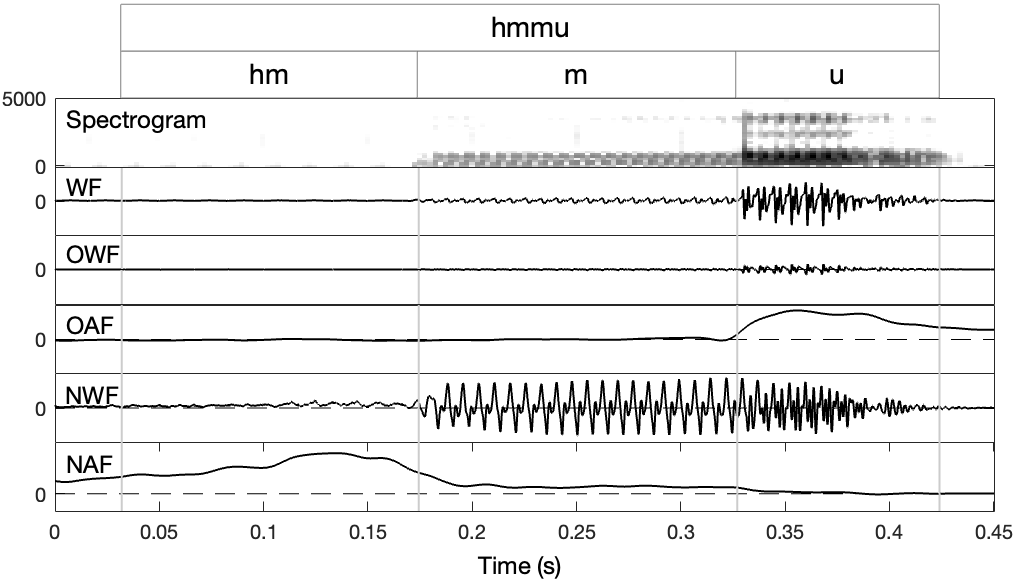
\includegraphics[width=.48\textwidth]{figures/a13ShinoharaHussainAmelot-img003.png}
}
\subfigure[\textit{hnnu} ‘horn’\label{fig:shinohara:3b}]{
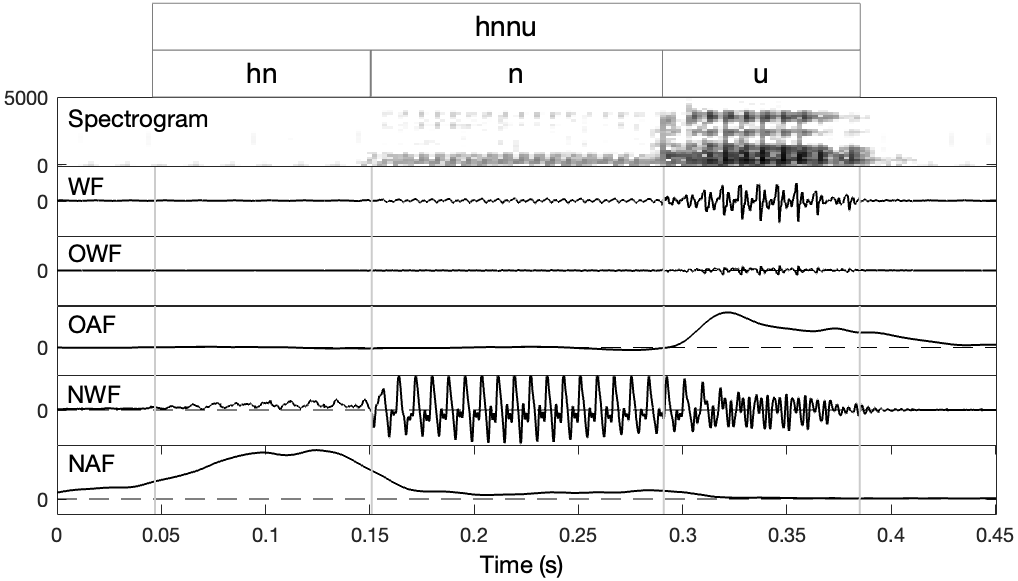
\includegraphics[width=.48\textwidth]{figures/a13ShinoharaHussainAmelot-img004.png}
}
\subfigure[\textit{mma} ‘mother’\label{fig:shinohara:3c}]{
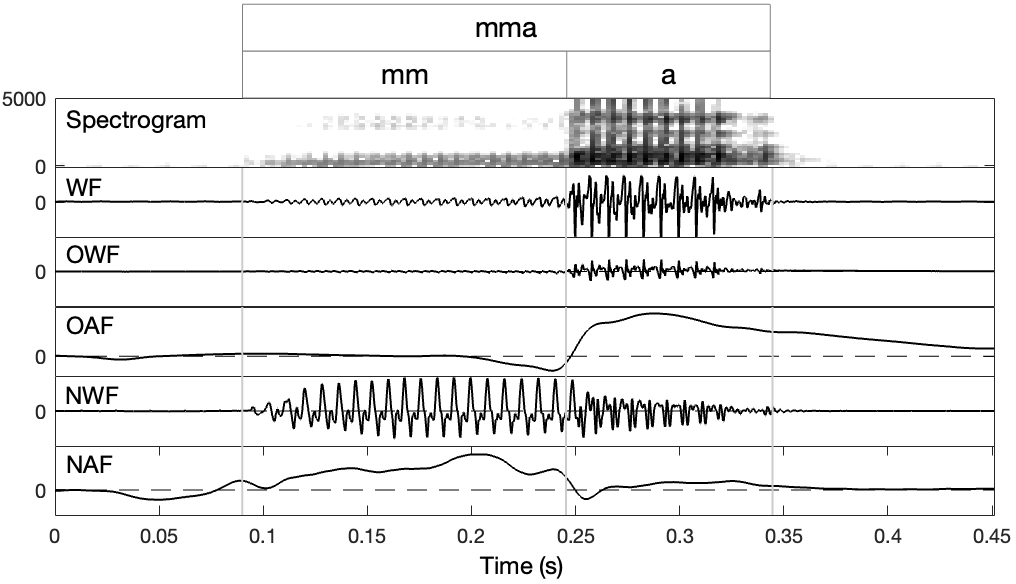
\includegraphics[width=.48\textwidth]{figures/a13ShinoharaHussainAmelot-img005.png}
}
\subfigure[\textit{nna} ‘spiral shell’\label{fig:shinohara:3d}]{
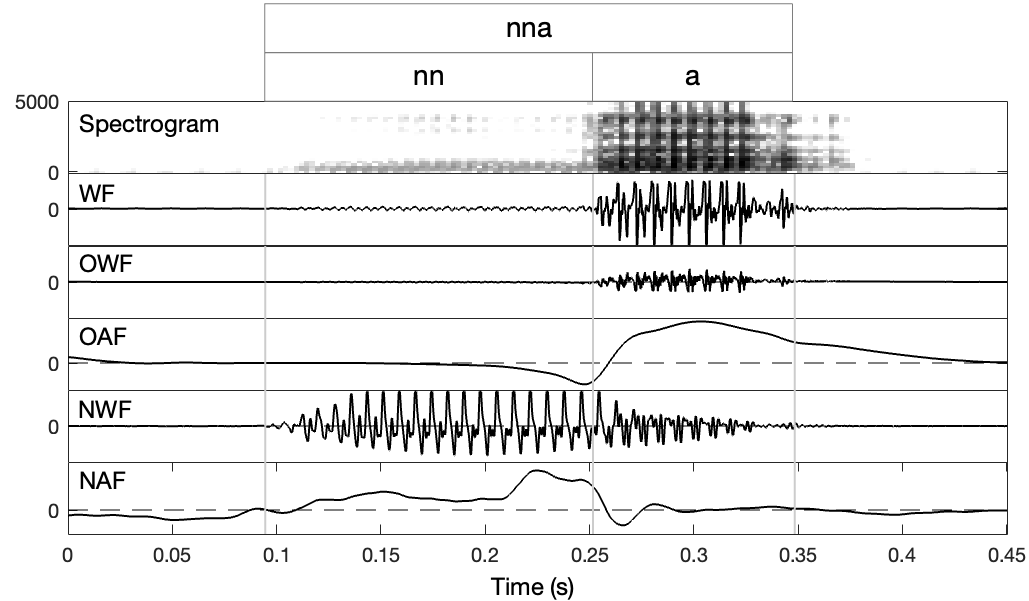
\includegraphics[width=.48\textwidth]{figures/a13ShinoharaHussainAmelot-img006.png}
}
\caption{\label{fig:shinohara:3}Spectrograms and waveforms of voiceless and voiced nasals. OWF = oral waveform, NWF = nasal waveform, OAF = oral airflow (L/sec), NAF = nasal airflow (L/sec)}
\end{figure}

\newpage
We next present the oral and nasal airflow patterns that differentiate voiceless and voiced nasals of the near-minimal pair words. The patterns are represented in \textit{z}-score from the mean of the quantity of the flow in graphs showing normalised duration (in \%). In \figref{fig:shinohara:4}, the “Voiceless interval” refers to the acoustically voiceless part preceding the voiced part in voiceless nasal geminates. In the same figure, the “Voiced interval” refers either to the voiced part of voiceless nasal geminates, the entire period of voiced geminate nasals or the entire period of singleton nasals.

At the onset of the voiced interval, there is no clear difference in oral airflow between voiceless and voiced nasals. However, differences in oral airflow curves at the offset of the voiced interval can be observed between bilabial and alveolar nasals. Faster oral flow transitions are recognised in bilabials. Nevertheless, a clear difference in nasal flow patterns between voiceless and voiced intervals can be observed. Nasal flow gradually rises during the voiceless interval and then decreases while approaching the onset of the voiced interval, while voiced nasals and voiced parts of voiceless nasal geminates show stable nasal flow.

\tabref{tab:13:sm1} (in the Supplementary materials) displays the pairwise comparisons of different types of nasals. The nasal airflow was able to differentiate several pairs, including voiceless and voiced nasals (e.g., \textit{hmm} vs. \textit{hnn}, \textit{hmm} vs. \textit{mm}), but no significant differences were found in nasal airflow for the voiced nasals (e.g., \textit{m} vs. \textit{mm}). The oral airflow distinguished \textit{hmm} vs. \textit{n} (estimate 0.9872, \textit{t} =5.958, \textit{p} < 0.001) and \textit{hnn} vs. \textit{n} (estimate 0.8785, \textit{t} = 5.523, \textit{p} < 0.001) in addition to oral pairs with different places of articulation (e.g., \textit{m} vs \textit{n}). No other significant differences were observed in voiceless and voiced nasals in oral airflow.


\begin{figure}
\subfigure[oral]{
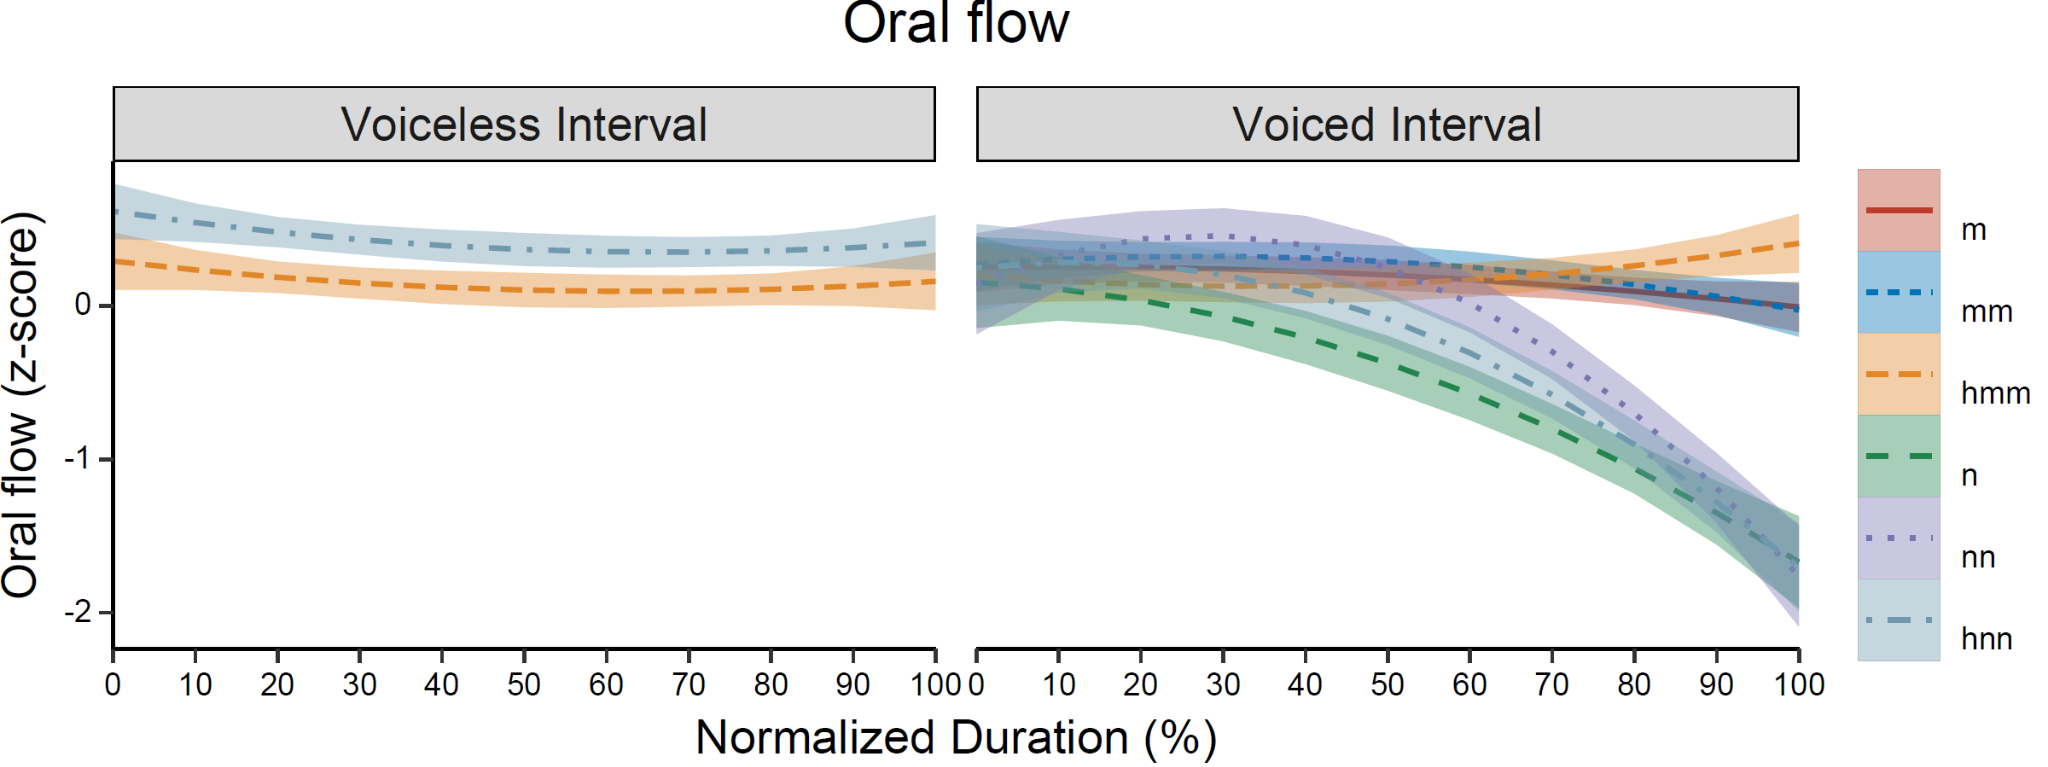
\includegraphics[width=.95\textwidth]{figures/a13ShinoharaHussainAmelot-img007.png}
}
\subfigure[nasal]{
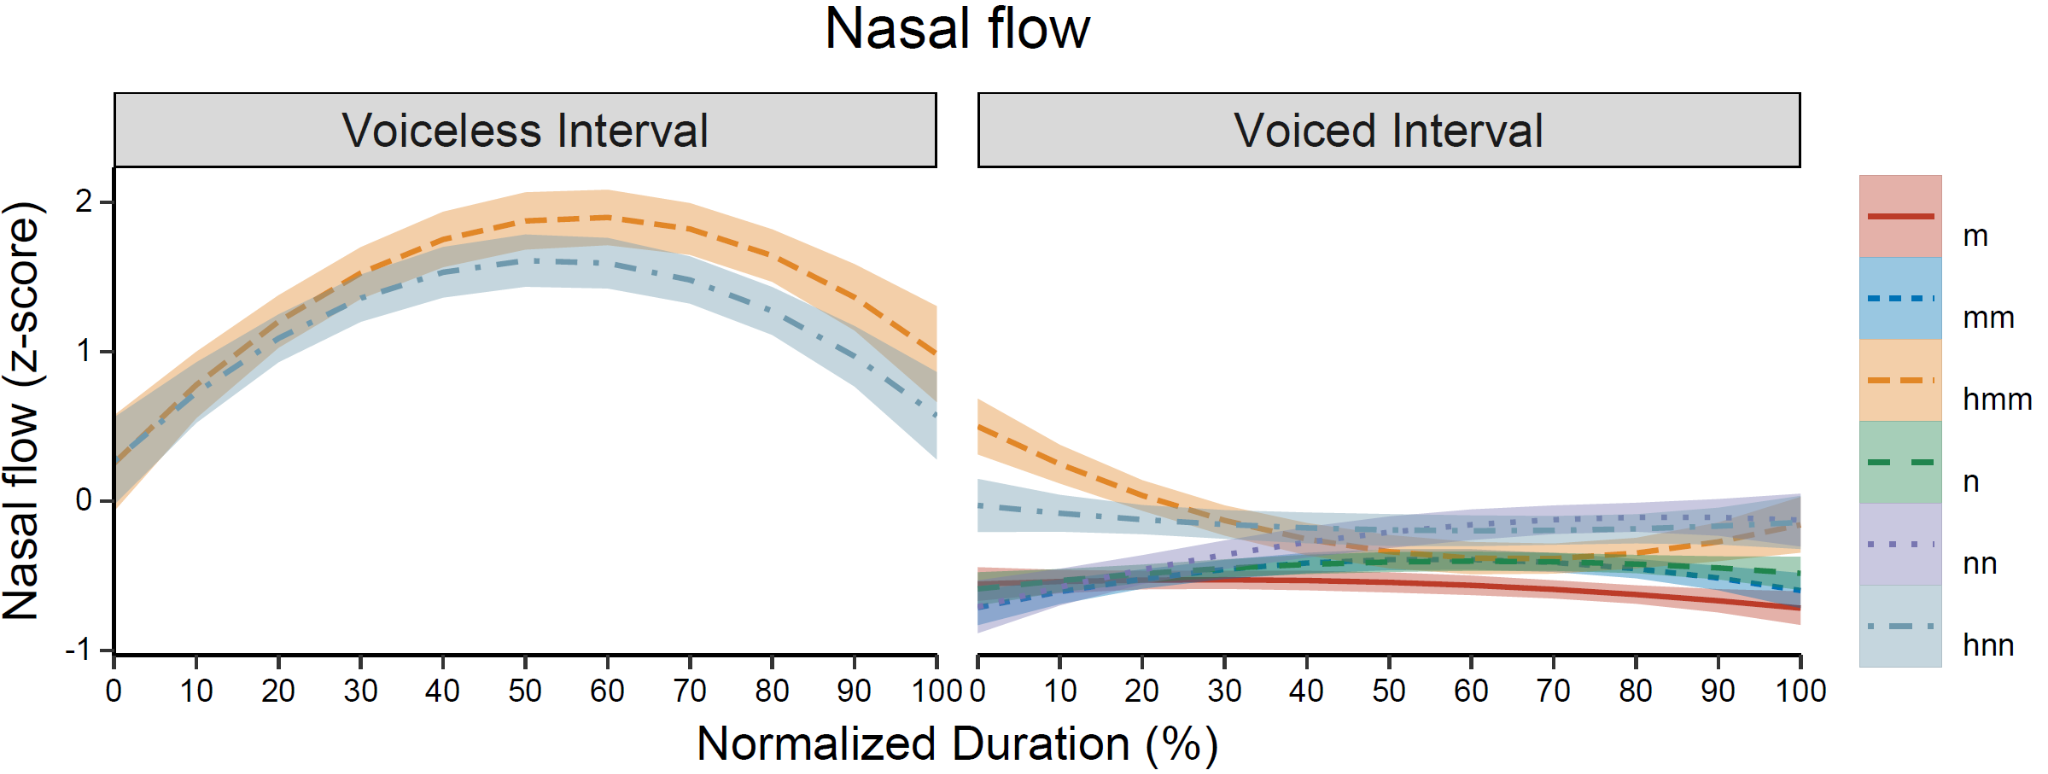
\includegraphics[width=.95\textwidth]{figures/a13ShinoharaHussainAmelot-img008.png}
}
\caption{\label{fig:shinohara:4}Smoothed curves of oral (top) and nasal (bottom) airflows. Note that \textit{z}-scores of the voiceless interval and those of the voiced interval are independent with respect to each other}
\end{figure}

\subsection{Durational characteristics of voiceless nasal geminates in Ikema}
\label{sec:shinohara:4.2}
In this section, we compare the proportions of voiceless and voiced intervals in Ikema voiceless nasals and analyse the phonological length of voiceless nasal geminates. To achieve the latter, we have included words with different mora counts and measured the entire word durations. The duration of each item is averaged over three tokens from each of the ten speakers (see \sectref{sec:shinohara:3.2} for variable token numbers). The acoustic duration of each segment of all the test words is shown in \figref{fig:shinohara:5}. Voiceless nasal geminates in \figref{fig:shinohara:5} are further divided into voiceless frication and voiced nasal parts.

The duration of the voiceless part of voiceless initial geminates is found to be shorter than the following voiced part. Specifically, the voiceless part had an average duration of 106~ms (SD: 6.8~ms). This was 37.5~\% of the whole duration of the geminate, which had an average overall duration of 282~ms (SD: 17.3~ms). The duration of the voiced initial geminates was on average 198~ms, which accounted for 70~\% of the whole voiceless geminate duration. 

Next, we assess the phonological length of the test words containing voiceless nasals by comparing them to other words with varying mora counts (see \tabref{tab:shinohara:7} for mora count of each test word). Each bar in \figref{fig:shinohara:5} represents the average total duration of the test words. According to the hypothesis of moraic isochrony at the word level in Ikema, words with the same mora count are expected to have similar duration (\citealt{ShinoharaFujimoto2018}). Conversely, words with different mora counts are predicted to have different durations. As such, we have expected that four-mora words (\textit{kannai} ‘thunder’ and \textit{hammai} ‘food’) would be the longest, followed by the three-mora word (\textit{maffa} ‘pillow’). Also, according to the hypothesis, there should be no big difference in duration among the two-mora words, which constitute a group of the most numerous words, and the two-mora words would be shorter than the three-mora word.

Pairwise comparisons of the overall durations of all words revealed that among the pairs of two-mora words, the significant differences always included a word with a voiceless nasal (\tabref{tab:13:sm2}), with the latter being longer. For example, \textit{ana} and \textit{hnna} exhibited differences even though they are both two-mora words, while \textit{ana} and \textit{mma} did not show a difference. Four-mora test words (\textit{hammai} and \textit{kannai}) did not exhibit a statistically significant difference from the three-mora test word (\textit{maffa}).\footnote{In this particular case, however, note that both of our four-mora test words have two (heavy) syllables which might have influenced the results (i.e., some degree of syllabic isochrony might also be implied).} The word \textit{hnna} [n̥na] ‘rope,’ which had fewer tokens than others, did not exhibit any statistically significant difference from longer words such as \textit{maffa} or \textit{kannai}. The other words with a voiceless nasal and all the other two-mora words were shorter than the three-mora word \textit{maffa}. 

  
\begin{figure}
% 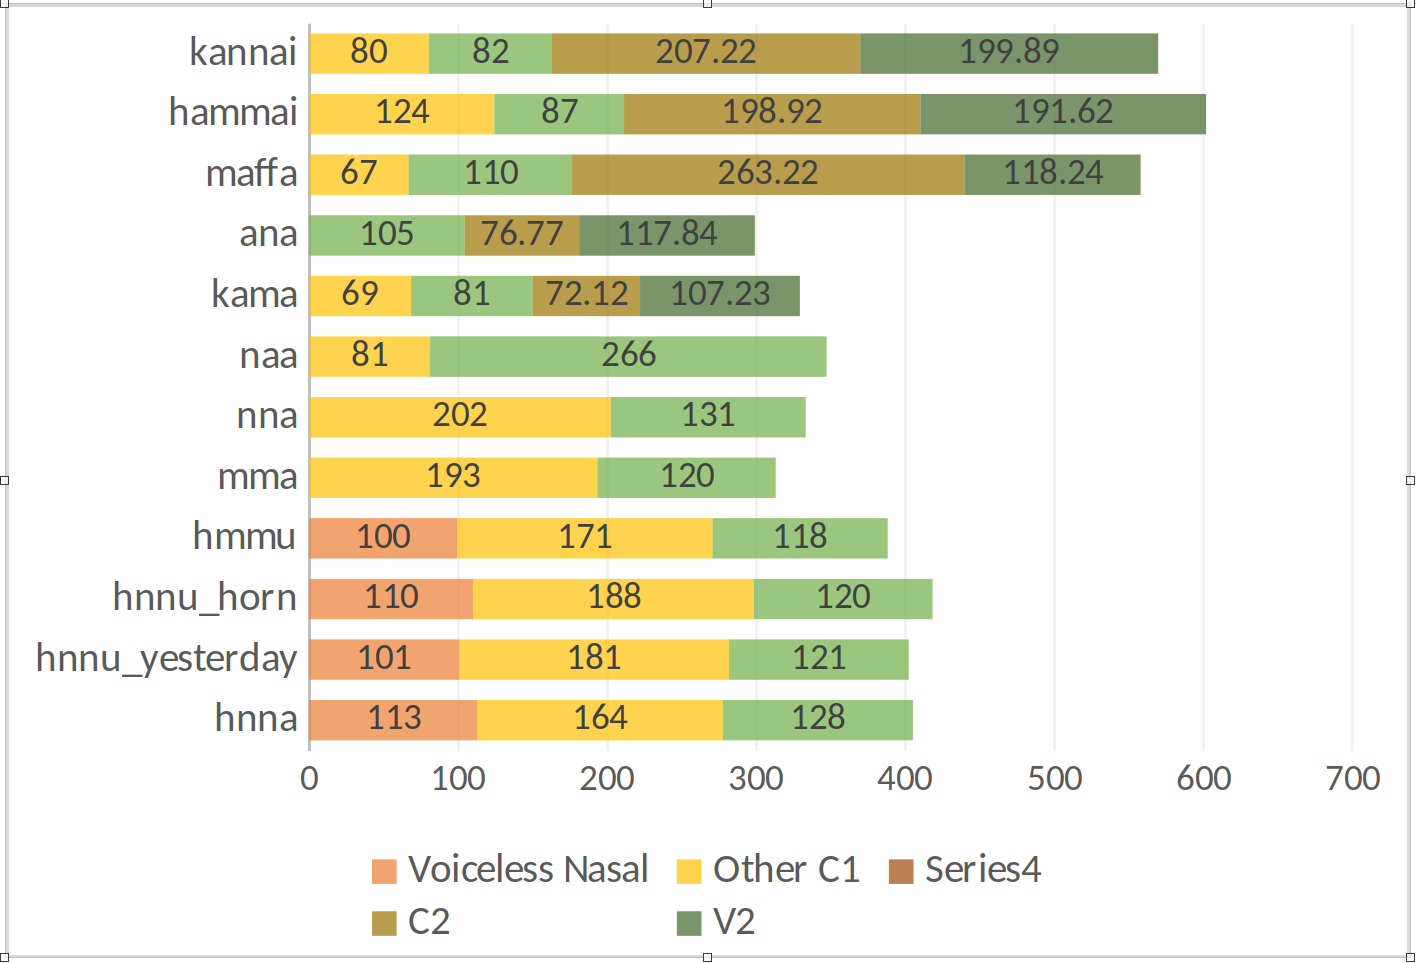
\includegraphics[width=\textwidth]{figures/shinohara_obj2.png}
    \begin{tikzpicture}
        \begin{axis}[
            xbar stacked,
            width  = .8\textwidth,
            height = .6\textheight,
            axis lines*=left,
            xmajorgrids,
            bar width = 10pt,
            xmin=0,
            xmax=700,
            symbolic y coords={
                hnna,
                hnnu\_yesterday,
                hnnu\_horn,
                hmmu,
                mma,
                nna,
                naa,
                kama,
                ana,
                maffa,
                hammai,
                kannai,
            },
%             nodes near coords,
            ytick=data,
            legend style={at={(0,0)},anchor=south west,font=\footnotesize},
            legend columns=5,
        ]
        \addplot+[lsDarkOrange] plot coordinates {
            (0,kannai)
            (0,hammai)
            (0,maffa)
            (0,ana)
            (0,kama)
            (0,naa)
            (0,nna)
            (0,mma)
            (100,hmmu)
            (110,hnnu\_horn)
            (101,hnnu\_yesterday)
            (113,hnna)
        };
        \addplot+[lsYellow] plot coordinates {
            (80,kannai)
            (124,hammai)
            (67,maffa)
            (0,ana)
            (69,kama)
            (81,naa)
            (202,nna)
            (193,mma)
            (171,hmmu)
            (188,hnnu\_horn)
            (181,hnnu\_yesterday)
            (164,hnna)
        };
        \addplot+[lsLightGreen] plot coordinates {
            (82,kannai)
            (87,hammai)
            (110,maffa)
            (105,ana)
            (81,kama)
            (266,naa)
            (131,nna)
            (120,mma)
            (118,hmmu)
            (120,hnnu\_horn)
            (121,hnnu\_yesterday)
            (128,hnna)
        };
        \addplot+[lsLightOrange] plot coordinates {
            (207,kannai)
            (199,hammai)
            (263,maffa)
            (77,ana)
            (72,kama)
            (0,naa)
            (0,nna)
            (0,mma)
            (0,hmmu)
            (0,hnnu\_horn)
            (0,hnnu\_yesterday)
            (0,hnna)
        };
        \addplot+[lsDarkGreenTwo] plot coordinates {
            (200,kannai)
            (192,hammai)
            (118,maffa)
            (118,ana)
            (107,kama)
            (0,naa)
            (0,nna)
            (0,mma)
            (0,hmmu)
            (0,hnnu\_horn)
            (0,hnnu\_yesterday)
            (0,hnna)
        };
        \legend{Voiceless Nasal,Other C1, V1, C2, V2}

        \end{axis}
  \end{tikzpicture}
\caption{\label{fig:shinohara:5}Average duration of segments in ms in the test words (typically three repetitions by ten speakers, but see \sectref{sec:shinohara:3.2} for the token number variability in some of the words). “Other C1” means an onset consonant of the initial syllable other than the voiceless nasal}
\end{figure}

\subsection{Non-temporal acoustic measurements at vowel onsets after voiceless and voiced nasal geminates and voiced singletons}
\label{sec:shinohara:4.3}
We have analysed the average values of f0 and H1*-H2* of the same subset of test words as used in the aerodynamic analysis. The values were \textit{z}-scored to normalise for individual pitch differences. In addition to these results, we present follow-up analyses to evaluate the effects of vowel quality, geminacy and lexical pitch-accent, because high vowels, geminate consonants and high tone might raise f0 independently of the voicing difference of the consonants.

The voiceless nasal \textit{hmm} showed the highest f0, followed by \textit{mm}, and then by other geminate nasals (\textit{hnn} and \textit{nn}) in the third place. Singletons (\textit{m} and \textit{n}) had the lowest f0. There were no clear differences in H1*-H2*. \tabref{tab:13:sm3} presents pairwise comparisons of f0, which show that several pairs with voiceless and voiced nasals were significantly different (e.g., \textit{hmm} vs. \textit{mm}). However, all the pairs distinguished by f0 either involved \textit{hmm} or were between singletons and geminates. The sound \textit{hnn} was only distinguished from the voiced singletons but not from the voiced geminates. It should be recalled that our selection of test words had some limitations. For instance, \textit{hmm} was followed by [u], while all the other words were followed by [a]. The ambiguity regarding whether the higher f0 in \textit{hmmu} is attributed to the voiceless onset nasal or the difference in vowel quality needs to be addressed.

We hypothesised that a closed vowel /u/ has a higher f0 than /a/, and that a vowel following a geminate consonant may also exhibit a higher f0 as compared to a vowel following a singleton onset (cf. \sectref{sec:shinohara:2.3}). In order to assess the impact of vowel quality and geminacy on the f0 results, we have performed LMER statistical analyses where the two segmentally homonymic words \textit{hnnu} (‘horn’; ‘yesterday’) were additionally included. These words had been excluded from the voicing comparison because the voiced counterpart \textit{nnu} was not recognised by our speakers. However, these words could be used for a vowel quality test with \textit{hnna}.

The analysis for vowel quality was conducted in two steps. First, we examined the impact of the vowel on the f0 results for the voiced singletons (\textit{maffa} and \textit{naa}). The results showed no significant difference between \textit{a} and \textit{aa} (t(54.6) = -1.355, \textit{p} = 0.1811). Second, we analysed the f0 results of the remaining geminates (\textit{hmmu, hnnu, hnna/hnnaa, mma, nna)}. Our results indicated that the f0 values of the vowels [a] and [u] gave different results, as demonstrated by the following statistical tests: \textit{a} -- \textit{aa} (t (169) = 3.188, \textit{p} = 0.0048), \textit{a -- u} (t (168) = -6.334, \textit{p} < 0.0001), and \textit{aa} -- \textit{u} (t (169) = -6.749, \textit{p} < 0.0001). Thus, we conclude that the higher f0 in \textit{hmmu} is likely due to its differing vowel quality, not due to the presence of a voiceless nasal.

We next compare the f0 values (\textit{z}-score normalised) of the singleton and geminate nasals. Our results indicate a significant difference between the f0 following a singleton and the f0 following a geminate nasal (\textit{t} (228) = 9.409, \textit{p} < 0.0001). We can therefore deduce that \textit{hnn} has higher f0 than \textit{m} and \textit{n} in our results rather because \textit{hnn} is a geminate not because it is voiceless.

Concerning the pitch-accent type, there is one word (\textit{mma} ‘mother’) that had been reported as having a different pitch-accent type (the C-type, the other test words having the B-type; see \tabref{tab:shinohara:7}). According to the description (\citealt{IgarashiEtAl2011} et seq.), the B-type accent on two-mora words is supposed to surface as the HL tone pattern and the C-type as the LH or HH pattern. Therefore, \textit{mma} is expected to show a higher tone than the B-type words on the second mora. However, only two speakers have produced a higher average f0 in the vowel part of \textit{mma} than in \textit{nna}. Therefore, there might be inter-speaker variation concerning lexical pitch-accent. The pitch-accents did not seem to exert much influence on the current f0 results.

After examining the potential factors influencing f0, it is concluded that geminacy and vowel height are the main factors which have an impact on the results. Therefore, the results did not support the hypothesis that the voiceless nasal is acoustically differentiated by f0 at the vowel onset. Furthermore, no significant differences have been found across the voiceless and the voiced nasals in the measured voice quality (H1*-H2*) (\tabref{tab:13:sm4}). 

\section{Summary and discussion}
\label{sec:shinohara:5}
This study has examined the aerodynamic and acoustic characteristics of word-initial voiceless and voiced nasal consonants in ten speakers of the endangered Ikema Miyako Ryukyuan dialect. To the best of our knowledge, voiceless nasals used as part of geminates have not been previously identified. The aerodynamic analysis has revealed that Ikema’s voiceless nasal geminates consist of a voiceless frication portion at the beginning, followed by a voiced nasal portion before the release. However, the voiceless portion is relatively shorter compared to that of the voiceless nasals in other languages. The acoustic investigation has shown that the voicing contrast is only evident during the voiceless interval of the voiceless geminates, as there have been no significant differences in the f0 or breathiness measures (H1*-H2*) at the onset of the following vowel between the voiceless and voiced nasal geminates. The voiceless nasal frication noise corresponds to oral fricative or affricate consonants, such as [f] or [ts], in cognate words in other Miyako Ryukyuan dialects (\sectref{sec:shinohara:1.3}). However, the perceptual cue of voiceless frication in Ikema’s voiceless nasal is short and non-robust. 

\subsection{Aerodynamic patterns}
\label{sec:shinohara:5.1}
\begin{sloppypar}
Nasal airflow distinguishes between voiceless and voiced nasals. During the voiceless interval, a significant rise in airflow has been observed. Dynamic airflow patterns also differ between the voiceless and voiced parts within a voiceless nasal sound. For voiceless nasals, airflow peaks around the middle of the interval and decreases towards the voiced part, whereas voiced nasals exhibit a consistent airflow. In a recent real-time magnetic resonance imaging analysis of voiceless nasals in Ikema by two speakers from the Nishihara area \citep{FujimotoEtAl2023}, a higher degree of velum lowering during the production of voiceless nasals was observed as compared to voiced geminate or singleton nasals. This pattern was consistent in both speakers. This distinct articulation may serve as a characteristic feature of voiceless nasals. Our present study reveals a substantial amount of airflow during the voiceless interval, which aligns with the aforementioned articulatory observation.
\end{sloppypar}

From a cross-linguistic perspective, our findings suggest that Ikema voiceless nasals conform to the Burmese type, rather than to the Angami type described in \citet{BhaskararaoLadefoged1991} (cf. \sectref{sec:shinohara:2.1}). Specifically, the nasal airflow continues through the closure release into the following vowel, and acoustic signals do not indicate the presence of a glottal fricative before the onset of the vowel as in Angami. However, there are differences from the Burmese airflow patterns found in \citet{ChirkovaEtAl2019}. The latter study characterised Burmese patterns (grouped with Mizo) as “pre-aspirated nasals,” which means that the voiceless nasals were accompanied by both oral and nasal flows and ended in voiced nasals. We do not observe any oral flow or aspiration noise from the oral cavity during the voiceless phase. Thus, the term “pre-aspirated nasals” is not adequate to describe Ikema voiceless nasals.

The Burmese data from \citet{BhaskararaoLadefoged1991} and \citet{ChirkovaEtAl2019} suggest that among Burmese speakers, some individuals may exhibit a loosened oral constriction during the articulation of voiceless nasals, while the majority of speakers maintain their oral constriction throughout this phase. In \citegen{BhaskararaoLadefoged1991} study, all speakers except one showed only nasal airflow during voiceless nasal production. The data from \citet{ChirkovaEtAl2019} do not necessarily contradict this pattern, as their airflow data are based on only three female speakers, and not all figures in their study indicate oral airflow during the voiceless nasal intervals. Hence, we propose that the presence or absence of oral airflow during or before the voiceless nasal period does not warrant a sub-classification of voiceless nasals into “pre-aspirated” and “not pre-aspirated,” because this may just reflect idiosyncratic variation.

Our data show another difference from the Burmese results reported by \citet{ChirkovaEtAl2019}. The amount of nasal airflow in their data was similar between voiceless and voiced nasals, whereas our data indicate weaker nasal flow during the voiced periods. However, in Chirkova et al.’s comparison, “voiceless nasals” included the voiced period, whereas we separate the phonetically voiceless period from the phonetically voiced one within the voiceless nasal geminate. 

\subsection{Durational correlates and timing patterns}
\label{sec:shinohara:5.2}
The voicing distinction between voiceless and voiced nasal geminates lies in a small portion of the nasal consonant. The average duration of the voiceless portion is 37.5~\% of the entire (geminate) duration in our study. This duration is significantly longer than the result obtained in a previous study of Ikema spoken in the Nishihara area, where the voiceless portion was only 16.5~\% of the duration (\citealt{ShinoharaFujimoto2018}, see below for the account of this discrepancy between the earlier and the current results). 

The voicing rate in Ikema is almost reversed as compared to the Burmese voiceless nasals, where the \textit{voiced} portion was reported around 30~\% in previous studies (25~\%-29~\% in \citealt{Dantsuji1984,Dantsuji1986}, 24~\% for male speakers across four places of articulation and 21~\% for female speakers across three places in \citealt{BhaskararaoLadefoged1991}, 33~\% in \citealt{ChirkovaEtAl2019} based on EGG).

In the case of Ikema, the voiced portion following the voiceless interval may be phonologically specified as voiced, as it has developed from a voiced nasal onset (\sectref{sec:shinohara:1.3}). Consequently, a long voicing period during the voiceless nasal geminates might be explained as an articulatory target, which could be distinct from the articulation of voiceless nasals in other languages. Furthermore, from a perceptual standpoint, as noted by \citet{OhalaOhala1993}, it would not be efficient to extend the voiceless interval to fill the geminate duration since it does not provide place cues or intense frication noise for indicating voicelessness. These weak acoustic cues of the voiceless nasal may have hindered the increase in the proportion of voicelessness in Ikema voiceless nasals.

Let us consider the timing patterns of voiceless nasals as geminate consonants. Word-initial voiceless nasal geminates have longer duration than singletons in our results, which confirms the finding in \citet[264]{ShinoharaFujimoto2018}. The current study also confirms that all two-mora words, including those starting with a voiceless nasal, are shorter than three-mora words. On the other hand, voiceless nasal geminates are longer than their voiced counterparts in our data, and the overall duration of words with an initial voiceless nasal is longer than that of other two-mora words.

In \citegen{ShinoharaFujimoto2018} study, they found that the test words starting with (voiceless and voiced) nasal geminates were shorter compared to the other two-mora words (see \figref{fig:shinohara:2}). However, in our current study, we observed a considerable difference in the duration of the voiceless interval, and this variation can be explained by several methodological differences. First, our voiceless intervals were segmented based on the waveform obtained through the airflow mask (see Sections~\ref{sec:shinohara:3.4} and~\ref{sec:shinohara:4.1} for details), which may have anticipated the acoustic frication noise which would have been captured by an external microphone. Second, it may be a dialectal difference between the varieties of Ikema. There is a possibility that the Nishihara variety, explored in the earlier study, is neutralising the voicing contrast in the initial nasal geminates. The third and presumably strongest effect might be potential hyper-articulation of the difference between voiced and voiceless nasals, which is related to the fact that the list of all test words was presented to speakers in a single block. In the current study, it was necessary to limit the time of wearing the airflow mask in hot and humid climates. The nasal geminate words in \citegen{ShinoharaFujimoto2018} acoustic study were instead mixed with other types of test words (a hundred words in total), which may have helped to avoid attracting the special attention of speakers to the voiceless nasals.

It should be noted that studies by \citet{LadefogedMaddieson1996} and \citet{ChirkovaEtAl2019} found longer durations for voiceless nasals as compared to voiced nasals in Burmese. There may be physiological explanations for this phenomenon, which may be explored in future studies to determine whether it is specific to the Burmese language or is a general characteristic of voiceless nasals.

\subsection{Non-temporal acoustic characteristics}
\label{sec:shinohara:5.3}
Previous studies have provided evidence that voiceless nasals can affect the fundamental frequency (f0) or spectral tilt of the following vowel. For instance, \citet{Maddieson1984} observed higher f0 values after voiceless nasals in Burmese, and \citet{Kirby2021} reported a similar effect in Eastern Khmu. Additionally, \citet{GogoiEtAl2018} identified breathy voice at the onset of the vowel following voiceless nasals in Miso. In our study, we have investigated the non-temporal properties, f0 and H1*-H2*, at the onset of the following vowel to examine voicing cues that could potentially signal the voicing contrast of nasals. A striking difference between Ikema and the previously studied languages is the absence of post-consonantal voicing cues. Our findings do not reveal any distinction between the vowel onsets following voiceless nasals and those following voiced nasals. This outcome was expected, given that Ikema is the only known language where the voiceless portion is consistently followed by an extended period of voicing. The long voiced interval may prevent the manifestation of voicing cues on the subsequent vowel.

We needed to conduct some additional tests since the real words did not always form perfect minimal pairs. For instance, the test words \textit{hmmu} ‘cloud’ and \textit{mma} ‘mother’ were contrasted not only in voicing but also in vowel quality. This made it impossible to directly observe the difference in f0 solely due to voicing. Among the additional tests, comparing the effect of geminate and singleton consonants on the f0 of the following vowel has revealed that all word-initial geminates, including voiceless nasals, induce higher f0 in the following vowel. Similar findings have been reported for other types of segments (\sectref{sec:shinohara:4.3}). In \citegen{HamzahEtAl2020} study, a higher f0 at the onset of the following vowel was found most evident for voiceless plosives in Kelantan Malay. And f0 also distinguished sonorant length differences (nasals and laterals). \citet{BurroniEtAl2021} reported similar effects in a few other languages. However, since their results were averaged over various segmental types, whether this is common across different types of obstruents and sonorants remained unclear. Our study has added empirical evidence for voiced and voiceless nasal consonants.

\subsection{Phonological predictions for voiceless nasal geminates}
\label{sec:shinohara:5.4}
Our study confirms that Ikema has developed the voiceless nasal geminates, which retain the voiceless, fricative, nasal and moraic characteristics of cognate forms found in other Miyako Ryukyuan dialects (e.g., [fumu] > [m̥mu], \sectref{sec:shinohara:1.3}). However, the voicelessness cue of these nasals may not be robust, as no enhancing cue has been identified in the following vowel. Based on these findings, there are potential scenarios for the future evolution of Ikema voiceless nasals. The weak acoustic cues may pose challenges in maintaining the voicing contrast in nasal geminates. The development of voiceless nasals from similar sequences (such as a voiceless segment followed by frication noise and a high vowel before a nasal, e.g., /tsImu/ ‘liver’) might be constrained, as is the case in other Miyako Ryukyuan dialects as well. It appears unlikely that Ikema will develop additional enhancing cues in the future, such as pitch or voice quality. The reason is that the presence of a long voiced interval may prevent the subsequent vowel from acquiring these features from the voiceless phonation, as long as the geminate is specified.

\begin{sloppypar}
Despite the intriguing sound features found in Ryukyuan languages, there have been only a few instrumental studies conducted on them thus far. The phonological and phonetic aspects of other dialects may exhibit ongoing changes, giving rise to forms that fall somewhere between, for instance, [fumu] and [m̥mu]. Undertaking such studies would offer further insight into the direction of these changes. Cross-dialectal comparisons are crucial for understanding their evolution. Cross-linguistic phonetic investigations are also important for comprehending the current status of these uncommon sounds. 
\end{sloppypar}

By investigating a unique case of word-initial voiceless nasal geminates in a Ryukyuan language, we contribute to the broader understanding of the diversity and complexity of sound systems in human languages. Further research on the phonological and phonetic aspects of uncommon speech sounds can shed light on the mechanisms behind their development and maintenance.


\section*{Acknowledgements}

We express our deep gratitude to the participants and the staff of NPO Kyuunu Hukarasha for their warm hospitality and cooperation in allowing us to use their facilities and conduct the experiments. We would like to acknowledge Thomas Pellard for providing valuable information regarding the accent types of the test words. Our sincere thanks go to the anonymous reviewers, the editors, Donna Erickson and Jeff Moore for their insightful comments. Any remaining errors are solely our responsibility. This project received partial funding from Labex EFL for Shigeko Shinohara and a Postdoctoral Travel Award from the Graduate School and Office of Postdoctoral Affairs at North Carolina State University, Raleigh, USA, for Qandeel Hussain.

\section*{Abbreviations}
\begin{multicols}{2}
\begin{tabbing}
\textsc{mmmm} \= accusative \kill
\textsc{top} \> topicalisation \\
NAF \> nasal airflow \\
NWF \> nasal waveform \\
OAF \> oral airflow \\
OWF \> oral waveform \\
WF \> waveform \\
SD \> standard deviation
\end{tabbing}
\end{multicols}

\begin{paperappendix}
\section{Supplementary materials: Aerodynamic and acoustic correlates of word-initial voiceless nasal geminates in Ikema Miyako Ryukyuan}
Original measurements used for the Supplementary materials reported below are available for download at \url{https://sdrive.cnrs.fr/s/sJy8rcW7FmAG2wP}

All the following analyses were performed using the \textit{lme4} package in R. Pairwise comparisons were conducted with \textit{emmeans} package. Consonant in the \textit{lmer} models refers to nasal consonants.


\begin{itemize}
\item[(i)] Models used in \tabref{tab:13:sm1}:
\item Oral airflow:
priming.lmer = lmer(OralFlowz {\textasciitilde} Consonant + (1{\textbar}Item) + (1{\textbar}Sp), data = 178)
\item Nasal airflow:
priming.lmer = lmer(NasalFlowz {\textasciitilde} Consonant + (1{\textbar}Item) +
(1{\textbar}Sp), data = 178)
\item \textit{emmeans}(priming.lmer, pairwise {\textasciitilde} Target\_consonant, lmer.df = ”satterthwaite”)
\end{itemize}

\begin{table}[H]
	\robustify{\bfseries}
	\begin{tabular}{l *2 {S[table-format=-.2] S[table-format=-1.2] S[table-format=<1.3]}}
		
		\lsptoprule
		& \multicolumn{3}{c}{Oral flow} & \multicolumn{3}{c}{ Nasal flow}\\\cmidrule(lr){2-4}\cmidrule(lr){5-7}
		Comparisons & {Est.} & {$t$} & {$p$} & {Est.} & {$t$} & {$p$}\\\midrule
		
		hmm vs. hnn & 0.10 & 0.66 & 0.985 & 0.70 & 4.77 & \bfseries < 0.001\\
		hmm vs. m & -0.23 & -1.39 & 0.731 & 2.00 & 13.40 & \bfseries < 0.001\\
		hmm vs. mm & 0.06 & 0.39 & 0.998 & 1.87 & 12.57 & \bfseries < 0.001\\
		hmm vs. n & 0.98 & 5.95 & \bfseries < 0.001 & 1.84 & 12.31 & \bfseries < 0.001\\
		hmm vs. nn & 0.55 & 3.34 & \bfseries 0.013 & 1.67 & 11.19 & \bfseries < 0.001\\
		hnn vs. m & -0.33 & -2.13 & 0.275 & 1.29 & 9.03 & \bfseries < 0.001\\
		hnn vs. mm & -0.04 & -0.27 & 0.999 & 1.17 & 8.17 & \bfseries < 0.001\\
		hnn vs. n & 0.87 & 5.52 & \bfseries < 0.001 & 1.13 & 7.90 & \bfseries < 0.001\\
		hnn vs. nn & 0.44 & 2.79 & 0.062 & 0.96 & 6.73 & \bfseries < 0.001\\
		m vs. mm & 0.29 & 1.84 & 0.440 & -0.12 & -0.86 & 0.955\\
		m vs. n & 1.21 & 7.59 & \bfseries < 0.001 & -0.16 & -1.12 & 0.869\\
		m vs. nn & 0.78 & 4.89 & \bfseries < 0.001 & -0.33 & -2.28 & 0.205\\
		mm vs. n & 0.92 & 5.75 & \bfseries < 0.001 & -0.03 & -0.26 & 0.999\\
		mm vs. nn & 0.48 & 3.04 & \bfseries 0.031 & -0.20 & -1.42 & 0.710\\
		n vs. nn & -0.43 & -2.70 & 0.079 & -0.16 & -1.15 & 0.855\\
		\lspbottomrule
	\end{tabular}
	\caption{Pairwise comparisons of oral and nasal flow amplitudes of word-initial voiceless and voiced nasals (\emph{maffa}, \emph{mma}, \emph{hmmu}, \emph{naa}, \emph{nna}, \emph{hnna}) (the values were $z$-score normalised; significant results in bold}
	\label{tab:13:sm1}
	\end{table}


\begin{itemize}
\item[(ii)] Models used in \tabref{tab:13:sm2}:
\item
Whole word duration:
priming.lmer = lmer(Duration\_total {\textasciitilde} Word + (1{\textbar}Item) + (1{\textbar}Sp), data = 324)
\item
\textit{emmeans} (priming.lmer, pairwise {\textasciitilde} Words, lmer.df = "satterthwaite")
\end{itemize}

{\robustify{\bfseries}
\begin{longtable}{l @{  vs. } l S[table-format=-3.2] S[table-format=-2.3] S[table-format=<1.3]}
\caption{Pairwise comparisons of word durations of all the words (significant results in bold)}
\label{tab:13:sm2}\\
        \lsptoprule
		\multicolumn{2}{l}{Comparisons} & {Est.} & {$t$} & {$p$}\\\midrule
        \endfirsthead
        \midrule
		\multicolumn{2}{l}{Comparisons} & {Est.} & {$t$} & {$p$}\\\midrule
        \endhead
		ana  &  hammai & -294.83 & -16.045 &  \bfseries < 0.001\\
		ana  &  hmmu & -113.35 & -5.99 &  \bfseries < 0.001\\
		ana  &  hnna & -200.38 & -5.26 &  \bfseries < 0.001\\
		ana  &  hnnu\_horn & -134.81 & -7.27 &  \bfseries < 0.001\\
		ana  &  hnnu\_yesterday & -115.86 & -6.30 &  \bfseries < 0.001\\
		ana  &  kama & -37.96 & -2.03 & 0.671\\
		ana  &  kannai & -264.36 & -14.38 &  \bfseries < 0.001\\
		ana  &  maffa & -278.43 & -15.15 &  \bfseries < 0.001\\
		ana  &  mma & -24.76 & -1.34 & 0.972\\
		ana  &  naa & -42.23 & -2.29 & 0.480\\
		ana  &  nna & -42.76 & -2.32 & 0.459\\
		hammai  &  hmmu & 181.47 & 9.87 &  \bfseries < 0.001\\
		hammai  &  hnna & 94.44 & 2.49 & 0.344\\
		hammai  &  hnnu\_horn & 160.01 & 8.90 &  \bfseries < 0.001\\
		hammai  &  hnnu\_yesterday & 178.96 & 10.04 &  \bfseries < 0.001\\
		hammai  &  kama & 256.86 & 14.15 &  \bfseries < 0.001\\
		hammai  &  kannai & 30.46 & 1.71 & 0.862\\
		hammai  &  maffa & 16.40 & 0.92 & 0.998\\
		hammai  &  mma & 270.06 & 15.15 &  \bfseries < 0.001\\
		hammai  &  naa & 252.60 & 14.17 &  \bfseries < 0.001\\
		hammai  &  nna & 252.06 & 14.14 &  \bfseries < 0.001\\
		hmmu  &  hnna & -87.02 & -2.28 & 0.491\\
		hmmu  &  hnnu\_horn & -21.45 & -1.16 & 0.991\\
		hmmu  &  hnnu\_yesterday & -2.50 & -0.13 & 1.000\\
		hmmu  &  kama & 75.39 & 4.03 &  \bfseries 0.003\\
		hmmu  &  kannai & -151.00 & -8.21 &  \bfseries < 0.001\\
		hmmu  &  maffa & -165.07 & -8.98 &  \bfseries < 0.001\\
		hmmu  &  mma & 88.59 & 4.82 &  \bfseries 0.001\\
		hmmu  &  naa & 71.12 & 3.87 &  \bfseries 0.007\\
		hmmu  &  nna & 70.59 & 3.84 &  \bfseries 0.008\\
		hnna  &  hnnu\_horn & 65.56 & 1.73 & 0.852\\
		hnna  &  hnnu\_yesterday & 84.51 & 2.23 & 0.524\\
		hnna  &  kama & 162.41 & 4.27 & \bfseries 0.001\\
		hnna  &  kannai & -63.98 & -1.69 & 0.870\\
		hnna  &  maffa & -78.04 & -2.06 & 0.648\\
		hnna  &  mma & 175.61 & 4.64 &  \bfseries < 0.001\\
		hnna  &  naa & 158.15 & 4.18 &  \bfseries 0.002\\
		hnna  &  nna & 157.61 & 4.17 &  \bfseries 0.002\\
		hnnu\_horn  &  hnnu\_yesterday & 18.95 & 1.05 & 0.996\\
		hnnu\_horn  &  kama & 96.85 & 5.29 &  \bfseries < 0.001\\
		hnnu\_horn  &  kannai & -129.54 & -7.20 &  \bfseries < 0.001\\
		hnnu\_horn  &  maffa & -143.61 & -7.98 &  \bfseries < 0.001\\
		hnnu\_horn  &  mma & 110.05 & 6.12 &  \bfseries < 0.001\\
		hnnu\_horn  &  naa & 92.58 & 5.15 &  \bfseries < 0.001\\
		hnnu\_horn  &  nna & 92.05 & 5.10 &  \bfseries < 0.001\\
		hnnu\_yesterday  &  kama & 77.90 & 4.29 &  \bfseries 0.001\\
		hnnu\_yesterday  &  kannai & -148.50 & -8.33 &  \bfseries < 0.001\\
		hnnu\_yesterday  &  maffa & -162.56 & -9.12 &  \bfseries < 0.001\\
		hnnu\_yesterday  &  mma & 91.10 & 5.11 &  \bfseries < 0.001\\
		hnnu\_yesterday  &  naa & 73.63 & 4.13 &  \bfseries 0.002\\
		hnnu\_yesterday  &  nna & 73.10 & 4.10 &  \bfseries 0.003\\
		kama  &  kannai & -226.40 & -12.47 &  \bfseries < 0.001\\
		kama  &  maffa & -240.46 & -13.25 &  \bfseries < 0.001\\
		kama  &  mma & 13.20 & 0.72 & 0.999\\
		kama  &  naa & -4.26 & -0.23 & 1.000\\
		kama  &  nna & -4.80 & -0.26 & 1.000\\
		kannai  &  maffa & -14.06 & -0.78 & 0.999\\
		kannai  &  mma & 239.60 & 13.44 &  \bfseries < 0.001\\
		kannai  &  naa & 222.13 & 12.46 &  \bfseries < 0.001\\
		kannai  &  nna & 221.60 & 12.43 &  \bfseries < 0.001\\
		maffa  &  mma & 253.66 & 14.23 &  \bfseries < 0.001\\
		maffa  &  naa & 236.20 & 13.25 &  \bfseries < 0.001\\
		maffa  &  nna & 235.66 & 13.22 &  \bfseries < 0.001\\
		mma  &  naa & -17.46 & -0.98 & 0.998\\
		mma  &  nna & -18.00 & -1.01 & 0.997\\
		naa  &  nna & -0.533 & -0.03 &  \bfseries 1.000\\
		\lspbottomrule
\end{longtable}}

\clearpage
\begin{itemize}
\item[(iii)] Models used in \tabref{tab:13:sm3}:
\item
F0:
priming.lmer = lmer(f0\_z {\textasciitilde} Consonant + (1{\textbar}Item) + (1{\textbar}Sp), data = 176)
\item
\textit{emmeans} (priming.lmer, pairwise{\textasciitilde} Consonant, lmer.df = "satterthwaite")
\end{itemize}

\begin{table}[H]
	\robustify{\bfseries}
	\begin{tabular}{l S[table-format=-1.2] S[table-format=-1.2] S[table-format=<1.3]}
		\lsptoprule
		Comparisons & {Est.} & {$t$} & {$p$}\\\midrule
		hmm vs. hnn & 0.56 & 5.11 & \bfseries <0.001\\
		hmm vs. m & 0.95 & 9.30 & \bfseries <0.001\\
		hmm vs. mm & 0.52 & 5.24 & \bfseries <0.001\\
		hmm vs. n & 0.92 & 9.50 & \bfseries <0.001\\
		hmm vs. nn & 0.62 & 6.33 & \bfseries <0.001\\
		hnn vs. m & 0.38 & 3.52 & \bfseries 0.007\\
		hnn vs. mm & -0.03 & -0.39 & 0.999\\
		hnn vs. n & 0.35 & 3.34 & \bfseries 0.012\\
		hnn vs. nn & 0.05 & 0.536 & 0.994\\
		m vs. mm & -0.42 & -4.28 & \bfseries < 0.001\\
		m vs. n & -0.03 & -0.32 & 0.999\\
		m vs. nn & -0.32 & -3.36 & \bfseries 0.012\\
		mm vs. n & 0.39 & 4.20 & \bfseries < 0.001\\
		mm vs. nn & 0.09 & 1.01 & 0.912\\
		n vs. nn & -0.29 & -3.23 & \bfseries 0.018\\
		\lspbottomrule
	\end{tabular}
	\caption{Pairwise comparisons of f0 of word-initial voiceless and voiced nasals (the values were $z$-score normalised; significant results in bold)}
	\label{tab:13:sm3}
\end{table}

\clearpage
\begin{itemize}
\item[(iv)] Models used in \tabref{tab:13:sm4}:
\item
H1*-H2*:
priming.lmer = lmer(H1H2c\_z {\textasciitilde} Consonant + (1{\textbar}Item) + (1{\textbar}Sp), data = 176)
\item
\textit{emmeans} (priming.lmer, pairwise{\textasciitilde} Consonant, lmer.df = "satterthwaite")
\end{itemize}

\begin{table}[H]
	\begin{tabular}{l S[table-format=-1.2] S[table-format=-1.2] S[table-format=1.3]}
		\lsptoprule
		Comparisons & {Est.} & {$t$} & {$p$}\\\midrule
		hmm vs. hnn & -0.05 & -0.26 & 0.999\\
		hmm vs. m & 0.01 & 0.09 &1.000\\
		hmm vs. mm & 0.14 & 0.72 &0.978\\
		hmm vs. n & -0.05 & -0.27 &0.999\\
		hmm vs. nn & 0.22 & 1.08 &0.885\\
		hnn vs. m & 0.07 & 0.35 &0.999\\
		hnn vs. mm & 0.20 & 0.94 &0.932\\
		hnn vs. n & 0.01 & 0.02 &1.000\\
		hnn vs. nn & 0.28 & 1.28 &0.794\\
		m vs. mm & 0.13 & 0.64 &0.987\\
		m vs. n & -0.07 & -0.37 &0.999\\
		m vs. nn & 0.20 & 1.01 &0.915\\
		mm vs. n & -0.20 & -1.05 &0.897\\
		mm vs. nn & 0.07 & 0.36 &0.999\\
		n vs. nn & 0.27 & 1.45 &0.692\\
		\lspbottomrule
	\end{tabular}
	\caption{Pairwise comparisons of H1*-H2* of word-initial voiceless and voiced nasals (the values were $z$-score normalised; significant results in bold)}
	\label{tab:13:sm4}
\end{table}
\end{paperappendix}
\sloppy\printbibliography[heading=subbibliography,notkeyword=this]
\end{document}
